% !TEX root = ../main.tex
\chapter{Thiết lập thực nghiệm và đánh giá hệ thống}
\label{Chapter4}

\par\noindent\rule{\textwidth}{0.4pt}\par

\section{Mục tiêu và câu hỏi đánh giá}

Chương 3 đã trình bày ConferenceSpace theo ba lớp trách nhiệm: nghiệp vụ cốt lõi, thuật toán xác định có thể kiểm chứng và AI hỗ trợ. Chương này trả lời câu hỏi tổng quát: trong điều kiện thử nghiệm, mỗi lớp thực hiện trách nhiệm được giao đến mức nào? Các nhóm bằng chứng được phân tách theo bản chất của từng tác vụ thay vì dùng một thước đo chung:

\begin{itemize}
  \item \textbf{Lớp nghiệp vụ cốt lõi:} nhóm dùng công cụ k6 để kiểm thử chịu tải HTTP và giám sát mức sử dụng tài nguyên. Phép đánh giá xác định hiệu năng và khả năng chịu tải của hệ thống trong các kịch bản thử nghiệm.
  \item \textbf{Lớp thuật toán:} nhóm đánh giá chức năng đối sánh phản biện viên và phát hiện xung đột lợi ích. Go microbenchmark đo trực tiếp thời gian xử lý và mức sử dụng bộ nhớ của thuật toán, không bao gồm chi phí HTTP, cơ sở dữ liệu và mạng. Thử nghiệm trên tập dữ liệu tổng hợp mô phỏng lược đồ (schema) Semantic Scholar đánh giá hành vi xếp hạng và phân công.
  \item \textbf{Lớp AI hỗ trợ:} nhóm đánh giá qua hai bước. Trước hết, các luồng AI xử lý dữ liệu đầu vào để tạo kết quả; sau đó, bộ kiểm thử TCA (Textual Claim-based Assessment) đánh giá các kết quả này theo độ trung thực (Truthfulness), độ phủ (Coverage) và Additionality. Với đầu ra có dữ liệu tham chiếu trực tiếp như Submission Autofill, chương sử dụng các chỉ số đối sánh như Exact Match, ROUGE và F1. Với Chatbot Agent, chương thử nghiệm thủ công theo các kịch bản hội thoại để kiểm tra tỷ lệ gọi công cụ thành công, khả năng tuân thủ quyền truy cập và trải nghiệm luồng phản hồi.
  \item Cuối cùng, chương này dùng UAT để đo mức độ đáp ứng nhu cầu của người dùng ở ba vai trò: Tác giả, Phản biện viên và Chủ tọa.
\end{itemize}

Cách tiếp cận này không quy toàn bộ lớp AI về một kết luận chung về độ tin cậy. Mỗi phép đo chỉ hỗ trợ một nhận định cụ thể: kiểm thử tải HTTP cho biết hành vi của các endpoint đã chọn; đánh giá thuật toán cho biết chất lượng theo nhãn tham chiếu hoặc chỉ số gián tiếp đã định nghĩa; TCA/NLI ước lượng mức độ bám bằng chứng; thử nghiệm hội thoại kiểm tra các kịch bản phân quyền; UAT phản ánh trải nghiệm của mẫu người dùng tham gia.

\subsection{Các lớp cần đánh giá}

Chương tổ chức việc đánh giá theo bốn nhóm bằng chứng, tương ứng với thiết kế hệ thống đã trình bày ở Chương 3.

\begin{PrismLongTable}
\begin{longtable}{|C{0.313\textwidth}|P{0.313\textwidth}|P{0.313\textwidth}|}
  \caption{Các lớp cần đánh giá}\LongTableCaptionSpace
  \hline
  \TableHeader{Lớp đánh giá}    &    \TableHeader{Đối tượng được kiểm tra}    &    \TableHeader{Vai trò trong luận điểm của đề tài} \\ \hline
  \endfirsthead
  \LongTableHeaderBorder
  \TableHeader{Lớp đánh giá}    &    \TableHeader{Đối tượng được kiểm tra}    &    \TableHeader{Vai trò trong luận điểm của đề tài} \\ \hline
  \endhead
  \LongTableFooterBorder
  \endfoot
  Nghiệp vụ cốt lõi     &     API của backend, cơ sở dữ liệu và các endpoint trong ba kịch bản tải     &     Đo hiệu năng của các đường xử lý đã chọn trong điều kiện thử nghiệm; không thay thế kiểm thử chức năng toàn bộ vòng đời hoặc thử nghiệm cô lập lỗi AI \\ \hline
  Thuật toán xác định, có thể kiểm chứng      &      Đối sánh phản biện viên, phát hiện xung đột lợi ích và các chỉ số chất lượng xếp hạng, phân công      &      Cung cấp bằng chứng rằng cơ chế xác định và có thể kiểm chứng xử lý các tác vụ đòi hỏi kết quả ổn định, có thể tái tạo và giải thích, qua đó tránh phụ thuộc vào tính ngẫu nhiên của mô hình AI tạo sinh \\ \hline
  Luồng xử lý AI hỗ trợ     &     Submission Autofill, Submission Gating, Reviewer Initial Analysis, Review Quality Auditor, Chair Decision Copilot và Chatbot Agent     &     Kiểm tra giá trị hỗ trợ của AI tại từng điểm nghẽn, đồng thời bảo đảm AI không thay thế quyết định học thuật \\ \hline
  Phản hồi người dùng      &      Khảo sát sau sử dụng theo các vai trò chính      &      Đối chiếu kết quả kỹ thuật với cảm nhận và nhu cầu thực tế của người dùng sau khi trải nghiệm hệ thống \\ \hline
\end{longtable}
\end{PrismLongTable}

Cách phân lớp này giúp chương tách biệt các loại kết luận. Hiệu năng tốt của backend không chứng minh AI đáng tin cậy; mức độ bám bằng chứng cao của luồng xử lý AI không chứng minh quyết định học thuật đúng; phản hồi tích cực của người dùng cũng không thay thế thử nghiệm định lượng.

\subsection{Câu hỏi đánh giá và phạm vi diễn giải}

Chương này tập trung trả lời các câu hỏi đánh giá sau:

\begin{PrismLongTable}
\begin{longtable}{|P{0.313\textwidth}|P{0.313\textwidth}|P{0.313\textwidth}|}
  \caption{Câu hỏi đánh giá và phạm vi diễn giải}\LongTableCaptionSpace
  \hline
  \TableHeader{Câu hỏi đánh giá}    &    \TableHeader{Nguồn bằng chứng}    &    \TableHeader{Tiêu chí diễn giải} \\ \hline
  \endfirsthead
  \LongTableHeaderBorder
  \TableHeader{Câu hỏi đánh giá}    &    \TableHeader{Nguồn bằng chứng}    &    \TableHeader{Tiêu chí diễn giải} \\ \hline
  \endhead
  \LongTableFooterBorder
  \endfoot
  Liệu hệ thống nghiệp vụ có đủ nhanh và ổn định trong điều kiện tải thử nghiệm hay không?     &     k6 kiểm thử tải, giám sát mức sử dụng tài nguyên và thống kê lỗi yêu cầu     &     Độ trễ p95, thông lượng, tỷ lệ lỗi và tài nguyên tiêu thụ trong các kịch bản CRUD, đối sánh phản biện viên và xung đột lợi ích \\ \hline
  Liệu đối sánh phản biện viên và xung đột lợi ích có thể chạy nhanh, có thể giải thích và có đường cơ sở so sánh hay không?      &      Go microbenchmark và thử nghiệm xếp hạng/phân công trên dữ liệu tổng hợp mô phỏng lược đồ (schema) Semantic Scholar      &      Thời gian xử lý, Hit@k, MRR, nDCG, độ phủ, mức độ đồng đều của phân công, tỷ lệ dùng lượt dự phòng và số ca tự gán \\ \hline
  Liệu các luồng xử lý AI có tạo đầu ra đủ bám bằng chứng để hỗ trợ người dùng hay không?     &     Bộ thực thi luồng xử lý, bộ thử nghiệm TCA, đối chiếu với chuẩn đã định sẵn và thử nghiệm hội thoại     &     Tỷ lệ hoàn tất, độ trễ, số token được xử lý, độ trung thực, độ phủ, Additionality, tính hợp lệ, tỷ lệ vừa bám nguồn vừa hợp lệ và khả năng tuân thủ quyền truy cập \\ \hline
  Liệu kết quả kỹ thuật có tương ứng với trải nghiệm người dùng hay không?      &      Khảo sát sau sử dụng trong chương này      &      Mức hài lòng, phản hồi định tính, điểm còn gây khó chịu và đề xuất cải thiện \\ \hline
\end{longtable}
\end{PrismLongTable}

Không phải chỉ số nào cũng có ngưỡng thành công được xác lập trước; vì vậy, chương không dùng nhãn hậu nghiệm \textit{đạt}/\textit{đạt một phần} như phán quyết chất lượng. Phần tổng hợp phân biệt ba trạng thái bằng chứng: \textit{có bằng chứng trực tiếp} khi phép đo đúng biến cần kết luận; \textit{chỉ có chỉ số gián tiếp} khi phép đo dùng nhãn thay thế, mẫu nhỏ hoặc bộ chấm tự động chưa hiệu chuẩn; và \textit{chưa đo} khi phép đánh giá cần thiết chưa được thực hiện. Điểm kiểm soát trong giao diện là đặc tính thiết kế; thực nghiệm chưa đo mức người dùng hiểu căn cứ, thực hiện ghi đè hoặc bị ảnh hưởng bởi thiên lệch tự động hóa.

\subsection{Liên kết với nhu cầu người dùng ở Chương 2}

Các nhóm đánh giá trên cung cấp bằng chứng trực tiếp cho một số biến kỹ thuật và bằng chứng gián tiếp cho một phần trong bốn nhu cầu đã rút ra ở Chương 2; chúng không đo đầy đủ hành vi hoàn thành nhiệm vụ, số bước thao tác, khả năng hiểu hạn chót hoặc hiệu quả thông báo.

\begin{PrismLongTable}
\begin{longtable}{|P{0.313\textwidth}|P{0.313\textwidth}|P{0.313\textwidth}|}
  \caption{Liên kết nhu cầu người dùng Chương 2 với đánh giá Chương 4}\LongTableCaptionSpace
  \hline
  \TableHeader{Nhu cầu từ Chương 2}    &    \TableHeader{Thành phần được đánh giá ở Chương 4}    &    \TableHeader{Ý nghĩa kiểm chứng} \\ \hline
  \endfirsthead
  \LongTableHeaderBorder
  \TableHeader{Nhu cầu từ Chương 2}    &    \TableHeader{Thành phần được đánh giá ở Chương 4}    &    \TableHeader{Ý nghĩa kiểm chứng} \\ \hline
  \endhead
  \LongTableFooterBorder
  \endfoot
  Giảm thao tác thủ công khi nộp bài     &     Submission Autofill và Submission Gating     &     Đo độ khớp siêu dữ liệu và kết quả của bộ ca kiểm tra luật; chưa đo số thao tác hoặc thời gian hoàn thành nhiệm vụ \\ \hline
  Giảm gánh nặng theo dõi cho Phản biện viên và Chủ tọa      &      Reviewer Initial Analysis, Review Quality Auditor, Chair Decision Copilot và Chatbot Agent      &      Đo độ trễ và mức độ bám nguồn theo bộ chấm; chưa đo tải nhận thức, khả năng xác định bước tiếp theo hoặc thời gian theo dõi \\ \hline
  Tăng kiểm soát rủi ro trong phân công và xung đột lợi ích     &     Đối sánh phản biện viên, thử nghiệm xung đột lợi ích và endpoint liên quan     &     Đo thời gian xử lý, khả năng truy hồi chủ đề và các chỉ số nội tại; chưa đo mức độ phù hợp của phản biện viên hoặc chất lượng phát hiện xung đột lợi ích đa tầng \\ \hline
  AI phải minh bạch và có thể ghi đè      &      Bộ thử nghiệm TCA, đối chiếu với chuẩn đã định sẵn, UAT và phần giới hạn thực nghiệm      &      Đo mức bám nguồn và sự tồn tại của điểm kiểm soát trong thiết kế; chưa đo khả năng người dùng hiểu căn cứ, thực hiện ghi đè hoặc tránh phụ thuộc vào gợi ý \\ \hline
\end{longtable}
\end{PrismLongTable}

Do đó, Chương 4 không chỉ báo cáo số liệu rời rạc. Vai trò của chương là tạo chuỗi bằng chứng từ yêu cầu người dùng, thiết kế hệ thống đến kết quả thực nghiệm, đồng thời chỉ ra rõ phần nào đã có bằng chứng và phần nào vẫn cần đánh giá thêm.

\par\noindent\rule{\textwidth}{0.4pt}\par

\section{Thiết lập thực nghiệm}

\subsection{Dữ liệu thực nghiệm}

Với lớp AI hỗ trợ, nhóm xây dựng tập dữ liệu thử nghiệm từ một tập con chọn lọc của ReviewRebuttal (Re2), bộ dữ liệu chứa hồ sơ phản biện bài báo qua nhiều giai đoạn từ OpenReview~\cite{ch4ref1}. Nhóm chỉ đánh giá các luồng AI trên dữ liệu nghiên cứu được phép sử dụng cho mục đích thử nghiệm; kết quả không chứng minh ConferenceSpace phù hợp để gửi bản thảo hoặc nội dung phản biện mật tới nhà cung cấp AI bên ngoài. Thay vì dùng toàn bộ dữ liệu gốc, nhóm chọn các bản ghi có đủ thông tin để tái tạo những luồng xử lý chính của ConferenceSpace: bài nộp, siêu dữ liệu, nhận xét phản biện, phản hồi hoặc bản tổng hợp nhận xét (metareview) khi có, cùng ngữ cảnh hội nghị. Cách chọn này giúp thử nghiệm đo đúng các luồng xử lý đã triển khai thay vì buộc hệ thống xử lý những bản ghi thiếu dữ liệu.

Bộ thực thi luồng xử lý được thử nghiệm trên 1.127 bài báo từ tám hội nghị hoặc chuyên đề khác nhau. Tập này được dùng để tạo đầu ra của các luồng AI, đồng thời ghi lại thời gian xử lý, số token tiêu thụ, trạng thái hoàn tất và các chỉ số đối sánh trực tiếp khi có dữ liệu tham chiếu rõ ràng. Trong số đó, 1.097 kết quả đủ điều kiện được đưa vào bộ thử nghiệm TCA để đánh giá chất lượng đầu ra dạng văn bản tự do. Hai nhóm chỉ số được đo trên các tập mẫu riêng: bộ thực thi luồng xử lý đo khả năng tạo đầu ra và vận hành, còn TCA đo mức độ bám bằng chứng của đầu ra đã tạo.


\begin{PrismLongTable}
\begin{longtable}{|C{0.313\textwidth}|C{0.313\textwidth}|C{0.313\textwidth}|}
  \caption{Thống kê tập dữ liệu thử nghiệm theo hội nghị và chuyên đề}\LongTableCaptionSpace
  \hline
  \TableHeader{Hội nghị / chuyên đề}    &    \TableHeader{Số lượng bài báo nộp}    &    \TableHeader{Tỷ lệ (\%)} \\ \hline
  \endfirsthead
  \LongTableHeaderBorder
  \TableHeader{Hội nghị / chuyên đề}    &    \TableHeader{Số lượng bài báo nộp}    &    \TableHeader{Tỷ lệ (\%)} \\ \hline
  \endhead
  \LongTableFooterBorder
  \endfoot
  ICLR 2023 TinyPapers     &     215     &     19,08\% \\ \hline
  UAI 2022 Conference      &      213      &      18,90\% \\ \hline
  CoRL 2023 Conference     &     191     &     16,95\% \\ \hline
  CoRL 2022 Conference      &      178      &      15,79\% \\ \hline
  MIDL 2023 Conference     &     111     &     9,85\% \\ \hline
  LOG 2022 Conference      &      82      &      7,28\% \\ \hline
  MIDL 2023 Short Paper Track     &     77     &     6,83\% \\ \hline
  IEEE ICIST 2024 Conference      &      60      &      5,32\% \\ \hline
  Tổng cộng     &     1.127     &     100,00\% \\ \hline
\end{longtable}
\end{PrismLongTable}

Ngoài bộ thực thi luồng xử lý, một số luồng dùng phép thử nghiệm riêng do khác biệt về bản chất đánh giá:

\begin{itemize}
  \item \textbf{Gợi ý chuyên đề trong Submission Autofill:} 48 trường hợp kiểm thử theo quy ước đầu ra, dùng để kiểm tra khả năng hoàn tất luồng và tính hợp lệ của mọi chuyên đề được gợi ý. Tập này chưa có nhãn chuyên gia để kết luận về tỷ lệ chọn đúng ở vị trí đầu tiên (Top-1) hoặc trong ba vị trí đầu (Top-3).
  \item \textbf{Submission Gating:} 8 trường hợp kiểm tra quy tắc cố định và 24 trường hợp kiểm tra cảnh báo nội dung do mô hình ngôn ngữ tạo ra. Tập này tách phần luật có kết quả kỳ vọng khỏi phần cảnh báo mềm chỉ đóng vai trò tín hiệu hỗ trợ.
  \item \textbf{Chatbot Agent:} 40 hội thoại thuộc 8 nhóm kịch bản, mỗi nhóm gồm 5 biến thể diễn đạt. Tập này dùng để đánh giá kết quả hội thoại, khả năng gọi công cụ, khả năng tuân thủ quyền truy cập và trải nghiệm luồng phản hồi.
\end{itemize}

Với lớp nghiệp vụ cốt lõi và lớp thuật toán, các mục sau trình bày chi tiết dữ liệu thử nghiệm. Kiểm thử hiệu năng backend dùng dữ liệu tổng hợp gồm 300 hội nghị, 15.000 bài nộp và 9.000 quan hệ phản biện viên--hội nghị. Đánh giá hành vi đối sánh dùng tập dữ liệu tổng hợp mô phỏng lược đồ (schema) Semantic Scholar gồm 60 hồ sơ tác giả và 2.565 bài báo.

\subsection{Môi trường thực nghiệm}

Nhóm thực hiện từng nhóm thực nghiệm trong môi trường phù hợp với loại hành vi cần đo. Bảng~\ref{tab:ch4-environments} tóm tắt môi trường, công cụ và tư liệu chính của từng nhóm.


\begin{PrismLongTable}
\begin{longtable}{|P{0.235\textwidth}|P{0.235\textwidth}|P{0.235\textwidth}|P{0.235\textwidth}|}
  \caption{Môi trường và tư liệu thực nghiệm}\label{tab:ch4-environments}\LongTableCaptionSpace
  \hline
  \TableHeader{Nhóm thực nghiệm}    &    \TableHeader{Môi trường/công cụ}    &    \TableHeader{Tư liệu đầu ra}    &    \TableHeader{Mục đích} \\ \hline
  \endfirsthead
  \LongTableHeaderBorder
  \TableHeader{Nhóm thực nghiệm}    &    \TableHeader{Môi trường/công cụ}    &    \TableHeader{Tư liệu đầu ra}    &    \TableHeader{Mục đích} \\ \hline
  \endhead
  \LongTableFooterBorder
  \endfoot
  Kiểm thử hiệu năng HTTP của backend     &     Backend gồm PostgreSQL, Neo4j, Redis và container API; k6 tạo tải HTTP     &     Bản tóm tắt JSON theo kịch bản, nhật ký tài nguyên và bản tóm tắt mức sử dụng tài nguyên     &     Đo độ trễ, thông lượng, tỷ lệ lỗi yêu cầu và mức tài nguyên tiêu thụ của lớp nghiệp vụ \\ \hline
  Go microbenchmark      &      Bộ kiểm thử Go chạy trực tiếp trên mã thuật toán      &      Tệp \textit{micro.txt} chứa thời gian mỗi thao tác (ns/op), bộ nhớ cấp phát mỗi thao tác (B/op) và số lần cấp phát bộ nhớ mỗi thao tác (allocs/op)      &      Tách thời gian xử lý và mức sử dụng bộ nhớ của thuật toán khỏi chi phí HTTP, cơ sở dữ liệu và mạng \\ \hline
  Hành vi truy hồi và phân công     &     Bộ kiểm thử Go chạy trên tập dữ liệu tổng hợp mô phỏng lược đồ (schema) Semantic Scholar, không gọi API trong quá trình đánh giá     &     Báo cáo Markdown/CSV về Hit@k, MRR, nDCG, độ phủ và mức độ đồng đều của phân công     &     Đo khả năng truy hồi hồ sơ tác giả theo chủ đề và các chỉ số nội tại của phân công trên dữ liệu tổng hợp; không đo mức độ phù hợp của phản biện viên \\ \hline
  Bộ thực thi luồng xử lý      &      Kiến trúc gồm bộ điều phối và các worker; mỗi tác vụ tương ứng với một bài nộp      &      Gói kết quả gồm ngữ cảnh nguồn, đầu ra của luồng xử lý, điểm kiểm tra theo giai đoạn, số token và thời gian xử lý      &      Tạo đầu ra của các luồng AI trên tập 1.127 bài \\ \hline
  Bộ thử nghiệm TCA     &     Worker sử dụng GPU L4 trên nền tảng đám mây, 2 CPU và 4 GB RAM; \CodeBreak{dleemiller/ModernCE-large-nli} với độ dài ngữ cảnh 8.192; \CodeBreak{Qwen/Qwen3.5-2B} và \CodeBreak{Qwen/Qwen3.5-0.8B} để chuẩn hóa mệnh đề~\cite{ch4ref2,ch4ref3}     &     Tệp JSONL chứa kết quả TCA theo từng bài và từng nhóm B1/B2/B3/B5     &     Đánh giá đầu ra dạng văn bản tự do theo độ trung thực (Truthfulness), độ phủ (Coverage) và Additionality \\ \hline
  Submission Gating và gợi ý chuyên đề      &      Đối chiếu với chuẩn đã định sẵn cho kiểm tra luật, cảnh báo nội dung và chuyên đề hợp lệ      &      Chỉ số tổng hợp, đầu ra đã chuẩn hóa và các trường hợp lỗi      &      Kiểm tra quy tắc cố định, phạm vi cảnh báo mềm và tính hợp lệ của chuyên đề được gợi ý \\ \hline
  Chatbot Agent     &     Thử nghiệm hội thoại theo 8 nhóm kịch bản, mỗi nhóm 5 biến thể     &     Bản ghi hội thoại, đánh giá thủ công, nhật ký gọi công cụ và thông tin thời gian     &     Đánh giá kết quả hội thoại, quyền truy cập, tỷ lệ gọi công cụ thành công và trải nghiệm luồng phản hồi \\ \hline
\end{longtable}
\end{PrismLongTable}

Bộ thực thi luồng xử lý dùng bộ định tuyến mô hình và Gemini 3.1 Flash Lite để tạo đầu ra. Bộ thử nghiệm TCA đọc lại gói kết quả đã lưu, dùng \CodeBreak{dleemiller/ModernCE-large-nli} để phân loại quan hệ bằng chứng--mệnh đề, \CodeBreak{Qwen/Qwen3.5-2B} để chuẩn hóa điểm cần lưu ý hoặc lập luận và \CodeBreak{Qwen/Qwen3.5-0.8B} cho bước phân loại hỗ trợ~\cite{ch4ref2,ch4ref3}. Việc tách hai môi trường giúp phân biệt khả năng tạo đầu ra với quy trình đánh giá đầu ra.

\subsection{Bộ dữ liệu tham chiếu và quy trình chấm điểm thử nghiệm}

Các luồng xử lý AI dùng ba kiểu đánh giá, tương ứng với mức độ sẵn có của dữ liệu tham chiếu:

\begin{itemize}
  \item \textbf{Đối chiếu trực tiếp với dữ liệu hoặc quy tắc tham chiếu:} Submission Autofill được so sánh với siêu dữ liệu bài nộp bằng Exact Match, ROUGE và F1. Submission Gating được kiểm tra bằng các trường hợp có sẵn phán quyết và mã luật kỳ vọng.
  \item \textbf{Đánh giá quan hệ mệnh đề--bằng chứng:} TCA đánh giá Reviewer Initial Analysis, Review Quality Auditor và Chair Decision Copilot bằng Truthfulness, Coverage và Additionality. Truthfulness ước lượng tỷ lệ mệnh đề có bằng chứng hỗ trợ; Coverage đo mức trùng khớp với nội dung tham chiếu do con người tạo; Additionality đo tỷ lệ mệnh đề được bộ chấm xem là có căn cứ nhưng không trùng trực tiếp với tham chiếu. Đây là phép chấm thăm dò tự động, chưa được hiệu chuẩn bằng nhãn chuyên gia và không tự xác nhận tính hữu ích học thuật của đầu ra.
  \item \textbf{Đánh giá theo hành vi hội thoại:} Chatbot Agent được kiểm tra qua các hội thoại mô phỏng theo vai trò Tác giả, Phản biện viên và Chủ tọa. Kết quả được chấm theo mức độ hoàn tất yêu cầu, mức độ bám dữ liệu nền tảng, khả năng tuân thủ quyền truy cập và khả năng kiểm soát phạm vi.
\end{itemize}

Tư liệu thô gồm các tệp JSON, JSONL và CSV của bộ thực thi luồng xử lý, TCA, Submission Gating, gợi ý chuyên đề trong Submission Autofill và Chatbot Agent. Các tệp này cho phép truy ngược từ số liệu tổng hợp đến từng tác vụ, phản hồi, cảnh báo hoặc phát hiện. Với thuật toán đối sánh, nhãn leave-one-out và các đường cơ sở chỉ phục vụ so sánh nội bộ trên dữ liệu tổng hợp; với khảo sát người dùng, phiếu trả lời là nguồn dữ liệu tham chiếu cho các thống kê mô tả theo vai trò.

\subsection{Kịch bản và chỉ số đánh giá}

Mỗi nhóm thực nghiệm trả lời một câu hỏi đánh giá riêng nhưng cùng tuân theo một khung phương pháp: xác định đầu vào và tiền điều kiện, mô tả thao tác hệ thống phải thực hiện, xác định đầu ra kỳ vọng, ghi nhận đầu ra thực tế dưới dạng tư liệu có thể truy xuất, sau đó tính chỉ số và xác định giới hạn diễn giải. Bảng~\ref{tab:ch4-scenario-map} cung cấp bản đồ tổng quan; phần chi tiết của từng nhóm được trình bày ngay sau bảng theo thứ tự các lớp hệ thống đã nêu ở Mục 4.1.

\begin{PrismLongTable}
\begin{longtable}{|P{0.20\textwidth}|P{0.24\textwidth}|C{0.14\textwidth}|P{0.20\textwidth}|C{0.12\textwidth}|}
  \caption{Tổng quan kịch bản đánh giá và chỉ số chính}\label{tab:ch4-scenario-map}\LongTableCaptionSpace
  \hline
  \TableHeader{Nhóm đánh giá}    &    \TableHeader{Câu hỏi cần trả lời}    &    \TableHeader{Quy mô mẫu}    &    \TableHeader{Chỉ số chính}    &    \TableHeader{Nơi trình bày kết quả} \\ \hline
  \endfirsthead
  \LongTableHeaderBorder
  \TableHeader{Nhóm đánh giá}    &    \TableHeader{Câu hỏi cần trả lời}    &    \TableHeader{Quy mô mẫu}    &    \TableHeader{Chỉ số chính}    &    \TableHeader{Nơi trình bày kết quả} \\ \hline
  \endhead
  \LongTableFooterBorder
  \endfoot
  Backend và giám sát mức sử dụng tài nguyên     &     Liệu hệ thống nghiệp vụ có ổn định dưới tải thử nghiệm hay không?     &     300 hội nghị; 15.000 bài nộp; 9.000 phản biện viên     &     Thông lượng, độ trễ p95, tỷ lệ lỗi, CPU/RAM     &     Mục 4.3 \\ \hline
  Go microbenchmark      &      Đối sánh phản biện viên và phát hiện xung đột lợi ích tiêu tốn bao nhiêu thời gian xử lý và bộ nhớ, không bao gồm chi phí HTTP, cơ sở dữ liệu và mạng?      &      Nhiều quy mô dữ liệu thử nghiệm thuật toán      &      \textit{ns/op}, \textit{B/op}, \textit{allocs/op}      &      Mục 4.4.1 \\ \hline
  Truy hồi hồ sơ tác giả và hành vi phân công     &     Jaccard có truy hồi quan hệ tác giả--chủ đề và thể hiện sự đánh đổi nội tại của thủ tục phân công hay không?     &     60 hồ sơ tác giả; 2.565 bài báo tổng hợp     &     Hit@k, MRR, nDCG, độ phủ đủ số phản biện viên, mức độ đồng đều, lượt dự phòng và ca tự gán     &     Mục 4.4.2 \\ \hline
  Bộ thực thi luồng xử lý      &      Liệu các luồng xử lý AI có tạo được đầu ra đáp ứng yêu cầu vận hành hay không?      &      1.127 bài      &      Tỷ lệ hoàn tất, độ trễ, số token và tính hợp lệ theo lược đồ (schema)      &      Mục 4.5 và 4.6 \\ \hline
  Phép chấm TCA thăm dò     &     Liệu đầu ra dạng văn bản tự do có bám bằng chứng nguồn hay không?     &     1.097 gói kết quả     &     Truthfulness, Coverage, Additionality, Validity     &     Mục 4.5 \\ \hline
  Submission Autofill      &      Liệu siêu dữ liệu có khớp dữ liệu tham chiếu và chuyên đề có hợp lệ hay không?      &      Siêu dữ liệu của 1.127 bài; 48 trường hợp chuyên đề      &      Exact Match, ROUGE, F1 và tỷ lệ chuyên đề không hợp lệ      &      Mục 4.5.3 \\ \hline
  Submission Gating     &     Liệu quy tắc cố định có cho kết quả đúng và cảnh báo mềm có giữ đúng phạm vi hay không?     &     8 trường hợp kiểm tra luật; 24 trường hợp cảnh báo nội dung     &     Độ chính xác của phán quyết, tỷ lệ nhận đúng mã luật, số lần chặn sai và số vi phạm quy tắc kiểm tra đầu ra     &     Mục 4.5.4 \\ \hline
  Chatbot Agent      &      Liệu trợ lý có tra cứu đúng, tuân thủ quyền truy cập và hoàn tất hội thoại hay không?      &      40 hội thoại; 8 nhóm kịch bản      &      Kết quả hội thoại, tỷ lệ gọi công cụ thành công, khả năng tuân thủ quyền truy cập và thời gian đến token đầu tiên (TTFT)      &      Mục 4.5.8 \\ \hline
  Khảo sát người dùng     &     Liệu kết quả kỹ thuật có tương ứng với trải nghiệm thực tế hay không?     &     Ba vai trò: Tác giả, Phản biện viên và Chủ tọa     &     Mức độ hài lòng, mức độ dễ thao tác và phản hồi định tính     &     Mục 4.7 \\ \hline
\end{longtable}
\end{PrismLongTable}

\subsubsection{Kịch bản đánh giá hiệu năng nghiệp vụ cốt lõi}

Nhóm đánh giá lớp nghiệp vụ cốt lõi trước vì các thao tác được chọn đi qua API và cơ sở dữ liệu của hệ thống. Kịch bản k6 đo độ trễ, tỷ lệ lỗi yêu cầu và mức sử dụng tài nguyên trên các đường HTTP đã xác định; phép đo không kiểm tra tính đúng chức năng của toàn bộ vòng đời và không cho phép suy rộng kết quả thành khả năng chịu tải của một hội nghị thực tế.

\textbf{Đầu vào.} Trước khi đo, nhóm khởi tạo hệ thống bằng bộ dữ liệu tổng hợp gồm 300 hội nghị, 50 bài nộp cho mỗi hội nghị và 30 phản biện viên cho mỗi hội nghị, tương ứng với 15.000 bài nộp và 9.000 quan hệ phản biện viên--hội nghị. Môi trường đo gồm container API, PostgreSQL, Neo4j và Redis. Cấu hình tải mặc định sử dụng 20 người dùng ảo trong 30 giây cho mỗi kịch bản k6.

\textbf{Các kịch bản và thao tác.} Ba kịch bản phản ánh các nhóm yêu cầu phổ biến nhất của nền tảng:

\begin{enumerate}
  \item \textbf{CRUD:} sau bước đăng nhập trong giai đoạn thiết lập, mỗi vòng lặp lần lượt liệt kê hội nghị, liệt kê bài nộp và tìm kiếm người dùng. Đây là ba endpoint chỉ đọc; kịch bản không tạo, cập nhật hoặc xóa bản ghi.
  \item \textbf{Đối sánh phản biện viên:} gọi endpoint \CodeBreak{reviewer-suggestions}. Kịch bản đo đường xử lý gợi ý qua API và không tự động phân công.
  \item \textbf{Xung đột lợi ích:} gọi endpoint kiểm tra xung đột lợi ích, bao gồm truy vấn quan hệ đồng tác giả trên Neo4j.
\end{enumerate}

Trong lúc chạy tải, bộ giám sát mức sử dụng tài nguyên lấy mẫu CPU và bộ nhớ theo từng giai đoạn và gắn nhãn \textit{crud}, \textit{matching} hoặc \textit{coi}.

\textbf{Đầu ra kỳ vọng.} Mỗi yêu cầu hợp lệ phải hoàn tất với mã trạng thái thành công; hệ thống phải ghi nhận số yêu cầu, thông lượng và các phân vị độ trễ. Bộ giám sát mức sử dụng tài nguyên phải tạo đủ chuỗi mẫu để so sánh mức tiêu thụ giữa API, PostgreSQL, Neo4j và Redis.

\textbf{Đầu ra thực tế và chỉ số.} Tư liệu chính gồm bản tóm tắt JSON theo từng kịch bản, nhật ký tài nguyên và bản tóm tắt mức sử dụng tài nguyên. Các chỉ số dùng để diễn giải gồm số yêu cầu, thông lượng, độ trễ trung vị, p90, p95, độ trễ tối đa, tỷ lệ lỗi, cùng mức sử dụng CPU và bộ nhớ trung bình hoặc cao nhất theo tiến trình hay container. Kết quả định lượng được trình bày tại Mục 4.3. Kiểm thử này chỉ đo tải trong điều kiện có kiểm soát, không thay thế kiểm thử chịu tải dài hạn hoặc phép ước lượng quy mô cho mọi môi trường triển khai.

\subsubsection{Kịch bản thuật toán đối sánh phản biện viên và xung đột lợi ích}

Sau khi đo hành vi đầu cuối qua API, chương tách chi phí thuật toán khỏi hành vi xếp hạng và phân công. Việc tách này cần thiết vì một endpoint đối sánh có độ trễ thấp vẫn có thể sử dụng thuật toán tốn tài nguyên; ngược lại, một thuật toán chạy nhanh vẫn có thể tạo danh sách xếp hạng kém chất lượng.

\textbf{Go microbenchmark.}

\begin{itemize}
  \item \textbf{Đầu vào:} bộ dữ liệu thử cho thuật toán đối sánh và xung đột lợi ích ở nhiều quy mô, từ vài chục đến vài nghìn bài nộp/phản biện viên. Kiểm thử chạy trực tiếp trên mã Go, không đi qua HTTP, tuần tự hóa hay cơ sở dữ liệu.
  \item \textbf{Thao tác:} mỗi phép kiểm thử được lặp 5 lần; hệ thống ghi \textit{ns/op}, \textit{B/op} và \textit{allocs/op}.
  \item \textbf{Đầu ra kỳ vọng:} xu hướng chi phí theo quy mô có thể quan sát được và so sánh giữa đối sánh phản biện viên với xung đột lợi ích.
  \item \textbf{Đầu ra thực tế và chỉ số:} tệp \textit{micro.txt} lưu kết quả của từng lần chạy; các chỉ số được tổng hợp tại Mục 4.4.1. Kết quả chỉ phản ánh thời gian xử lý và mức sử dụng bộ nhớ trong chương trình, không bao gồm chi phí HTTP, cơ sở dữ liệu và mạng.
\end{itemize}

\textbf{Đánh giá chất lượng xếp hạng và phân công.}

\begin{itemize}
  \item \textbf{Đầu vào:} tập dữ liệu tổng hợp \CodeBreak{testdata/s2\_snapshot.json} gồm 60 hồ sơ tác giả và 2.565 bài báo, mô phỏng lược đồ (schema) Semantic Scholar ở 8 lĩnh vực khoa học máy tính. Mỗi hồ sơ có ít nhất hai bài để hỗ trợ phương pháp giữ lại một bài làm truy vấn.
  \item \textbf{Thao tác xếp hạng:} với mỗi tác giả, một bài được giữ lại làm truy vấn; các tác giả còn lại được xếp hạng bằng Jaccard, \textit{overlap\_count} và phương pháp cơ sở ngẫu nhiên. Vị trí của tác giả gốc trong danh sách cho biết mức độ thuật toán truy hồi được liên kết chủ đề giữa bài và hồ sơ chuyên môn.
  \item \textbf{Thao tác phân công:} thuật toán gán tham lam được so sánh với phương pháp gán tuần tự và gán ngẫu nhiên bằng các chỉ số nội tại của phân công, vì chưa có nhãn tham chiếu cho phương án phân công tối ưu.
  \item \textbf{Đầu ra kỳ vọng:} phương pháp xếp hạng truy hồi hồ sơ tác giả gốc tốt hơn đường cơ sở ngẫu nhiên; phương pháp phân công không tạo ca tự gán; thử nghiệm đo được độ phủ, mức độ đồng đều và tỷ lệ sử dụng lượt dự phòng.
  \item \textbf{Đầu ra thực tế và chỉ số:} báo cáo Markdown/CSV và các bảng tại Mục 4.4.2, gồm Hit@k, MRR, nDCG@k, độ phủ, độ lệch chuẩn của số bài được phân công, hệ số Gini, điểm Jaccard trung bình, tỷ lệ dùng lượt dự phòng và số ca tự gán.
\end{itemize}

Microbenchmark và đánh giá hành vi cung cấp hai nhóm bằng chứng bổ sung cho nhau: microbenchmark đo thời gian xử lý của mã thuật toán, còn đánh giá hành vi đo khả năng truy hồi quan hệ tác giả--chủ đề và các chỉ số nội tại của phân công. Cả hai phép đánh giá đều không có nhãn về phản biện viên phù hợp hoặc dữ liệu phân công thực do Chủ tọa xác nhận; vì vậy, chúng không trả lời trực tiếp liệu gợi ý có đủ chất lượng để sử dụng trong vận hành hay không.

\subsubsection{Kịch bản tạo đầu ra và đánh giá luồng xử lý AI}

Lớp AI được đánh giá theo hai bước nối tiếp thay vì bằng một chỉ số duy nhất. Bước thứ nhất kiểm tra liệu luồng xử lý có tạo được đầu ra đáp ứng yêu cầu vận hành hay không. Bước thứ hai kiểm tra liệu đầu ra dạng văn bản tự do đã tạo có bám bằng chứng nguồn hay không. Việc tách bộ tạo đầu ra khỏi bộ đánh giá giúp báo cáo phân biệt khả năng vận hành với độ tin cậy của nội dung.

\textbf{Bộ thực thi luồng xử lý.}

\begin{itemize}
  \item \textbf{Đầu vào:} 1.127 bài từ tập ReviewRebuttal đã chọn lọc, có đủ bài nộp, siêu dữ liệu, nhận xét phản biện, phản hồi hoặc bản tổng hợp nhận xét (metareview) theo yêu cầu của từng luồng xử lý. Trong kiến trúc gồm bộ điều phối và các worker, mỗi tác vụ tương ứng với một bài nộp.
  \item \textbf{Thao tác:} bộ thực thi gọi luồng xử lý đã triển khai, đồng thời lưu ngữ cảnh nguồn, điểm kiểm tra của từng giai đoạn, đầu ra cuối cùng, số token và thời gian xử lý. Với Submission Autofill, hệ thống đối chiếu trực tiếp siêu dữ liệu được tạo với siêu dữ liệu tham chiếu.
  \item \textbf{Đầu ra kỳ vọng:} đầu ra tuân thủ lược đồ (schema); luồng xử lý hoàn tất hoặc ghi nhận lỗi có thể truy xuất; các trường có nhãn tham chiếu rõ ràng cho phép tính Exact Match, ROUGE hoặc F1.
  \item \textbf{Đầu ra thực tế và chỉ số:} gói kết quả JSON/JSONL/CSV của từng tác vụ. Các chỉ số vận hành gồm tỷ lệ hoàn tất, độ trễ và số token; các chỉ số đối sánh trực tiếp của Submission Autofill được trình bày tại Mục 4.5.3.
\end{itemize}

\textbf{Phép chấm TCA thăm dò.}

\begin{itemize}
  \item \textbf{Đầu vào:} 1.097 gói kết quả đủ điều kiện từ Reviewer Initial Analysis, Review Quality Auditor và Chair Decision Copilot. Bằng chứng đối chiếu gồm bài nộp, nhận xét phản biện hoặc bản tổng hợp nhận xét (metareview) tùy luồng xử lý.
  \item \textbf{Thao tác:} hệ thống trích mệnh đề từ đầu ra, ghép bằng chứng--mệnh đề, dùng NLI để gán trạng thái Truthfulness; Coverage và Additionality chỉ được tính trên các mệnh đề đã qua Truthfulness.
  \item \textbf{Đầu ra kỳ vọng:} mỗi mệnh đề có trạng thái bám nguồn có thể truy ngược; mỗi luồng xử lý có các điểm Truthfulness, Coverage, Additionality, Validity, tỷ lệ vừa bám nguồn vừa hợp lệ hoặc tỷ lệ rủi ro cao tương ứng.
  \item \textbf{Đầu ra thực tế và chỉ số:} JSONL theo từng bài và các bảng tại Mục 4.5.5--4.5.7.
\end{itemize}

Bộ thực thi tạo tập đầu ra thực nghiệm; TCA đọc lại tập này mà không tạo lại đầu ra. Cách tách này giữ riêng bằng chứng vận hành và bằng chứng về mức độ bám nguồn.

\subsubsection{Kịch bản đối chiếu đầu ra với chuẩn của Submission Autofill và Submission Gating}

Một số luồng AI cho phép đánh giá chặt chẽ hơn bằng cách đối chiếu đầu ra với chuẩn đã định sẵn vì có dữ liệu tham chiếu trực tiếp hoặc quy tắc kiểm tra cố định. Hai nhóm này được tách khỏi TCA vì phần cốt lõi có thể được đánh giá trực tiếp mà không cần chỉ số gián tiếp về quan hệ mệnh đề--bằng chứng.

\textbf{Submission Autofill.}

\begin{itemize}
  \item \textbf{Đầu vào siêu dữ liệu:} tệp PDF hoặc nội dung bài nộp cùng siêu dữ liệu tham chiếu của 1.127 bài.
  \item \textbf{Đầu vào gợi ý chuyên đề:} 48 trường hợp có danh sách chuyên đề hợp lệ của hội nghị đang xét.
  \item \textbf{Thao tác:} luồng xử lý trích xuất tiêu đề, tóm tắt, từ khóa, tác giả và các trường bắt buộc; với nhóm chuyên đề, luồng xử lý xếp hạng các chuyên đề trong danh sách cho phép.
  \item \textbf{Đầu ra kỳ vọng:} siêu dữ liệu gần với dữ liệu tham chiếu; mọi chuyên đề được gợi ý đều nằm trong danh sách hợp lệ; luồng xử lý hoàn tất.
  \item \textbf{Đầu ra thực tế và chỉ số:} gói kết quả siêu dữ liệu từ bộ thực thi và bản tóm tắt kết quả đối chiếu chuyên đề với chuẩn đầu ra. Các chỉ số gồm Exact Match của tiêu đề, F1 theo token của tiêu đề, ROUGE của tóm tắt, F1 của từ khóa, F1 của tác giả, tỷ lệ hoàn tất trường bắt buộc, tỷ lệ hoàn tất luồng và tỷ lệ chuyên đề không hợp lệ.
\end{itemize}

\textbf{Submission Gating.}

\begin{itemize}
  \item \textbf{Đầu vào kiểm tra luật:} 8 bộ dữ liệu thử được khởi tạo có kiểm soát. Mỗi bộ gồm nội dung bài hoặc tệp đầu vào, tập quy tắc áp dụng và cặp phán quyết kỳ vọng--mã luật. Ví dụ, bộ \textit{gating\_rule\_0002} chứa một tệp PDF đọc được với bốn tài liệu tham khảo, trong khi quy tắc yêu cầu tối thiểu sáu tài liệu.
  \item \textbf{Đầu vào cảnh báo nội dung:} 24 trường hợp nội dung cần cảnh báo mềm, không có quyền tự động loại bài.
  \item \textbf{Thao tác:} nhánh kiểm tra quy tắc cố định so sánh phán quyết thực tế và mã luật với kết quả kỳ vọng; nhánh kiểm tra nội dung tạo các cảnh báo mềm; hệ thống kiểm tra để bảo đảm không tạo trạng thái \textit{block} (chặn) tự động.
  \item \textbf{Đầu ra kỳ vọng:} kiểm tra luật trả đúng \textit{pass} (đạt), \textit{warn} (cảnh báo) hoặc \textit{block} (chặn) cùng đúng mã luật; nhánh kiểm tra nội dung chỉ tạo cảnh báo và giữ quyền quyết định cho người phụ trách.
  \item \textbf{Đầu ra thực tế và chỉ số:} \textit{tasks.jsonl} lưu đầu vào và đầu ra kỳ vọng; \textit{normalized\_rule\_findings.jsonl} lưu đầu ra thực tế; \textit{summary\_metrics.json} lưu độ chính xác phán quyết, tỷ lệ nhận đúng mã luật, số lần chặn sai, số phát hiện và số vi phạm quy tắc kiểm tra đầu ra.
\end{itemize}

Hai đánh giá này củng cố luận điểm thiết kế của đề tài: phần có quy tắc hoặc siêu dữ liệu rõ ràng cho phép đối chiếu trực tiếp; phần mang tính diễn giải học thuật phải giữ vai trò hỗ trợ và không được dùng để đưa ra phán quyết tự động.

\subsubsection{Kịch bản hội thoại của Chatbot Agent}

Nhóm không đánh giá Chatbot Agent như một mô hình trả lời mở hoặc trợ lý nghiên cứu. Phép đánh giá xem thành phần này là trợ lý của nền tảng, có trách nhiệm tiếp nhận yêu cầu theo vai trò, gọi công cụ nội bộ, trả lời dựa trên dữ liệu ConferenceSpace và tuân thủ ranh giới quyền truy cập.

\textbf{Đầu vào.} Nhóm dùng bộ dữ liệu khởi tạo để thiết lập một hội nghị giả lập với hai bài nộp, một Tác giả, một Phản biện viên và một Chủ tọa. Tám nhóm kịch bản được xác định trước, mỗi nhóm có năm biến thể diễn đạt, tổng cộng 40 hội thoại:

\begin{enumerate}
  \item Tác giả tra cứu trạng thái bài của chính mình.
  \item Tác giả tra cứu chuyên đề và siêu dữ liệu của bài do mình nộp.
  \item Chủ tọa yêu cầu tổng quan vận hành hội nghị.
  \item Phản biện viên kiểm tra phân công hoặc khối lượng công việc.
  \item Tác giả tra cứu thông tin công khai của hội nghị.
  \item Tác giả yêu cầu chi tiết bài của tác giả khác để kiểm tra ranh giới quyền truy cập.
  \item Tác giả yêu cầu nghiên cứu hoặc báo cáo ngoài phạm vi nền tảng.
  \item Chủ tọa yêu cầu báo cáo vận hành nhiều bước từ dữ liệu nội bộ.
\end{enumerate}

Mỗi kịch bản lưu sẵn vai trò, yêu cầu mẫu, dữ liệu khởi tạo cần có, công cụ kỳ vọng và tiêu chí chấm thủ công.

\textbf{Thao tác.} Bộ thực thi gửi yêu cầu bằng tài khoản tương ứng với từng vai trò, chờ trợ lý hoàn tất luồng phản hồi, rồi lưu bản ghi hội thoại, nhật ký gọi công cụ, thời gian đến token đầu tiên (TTFT), thời gian đến câu trả lời hoàn chỉnh đầu tiên, thời lượng luồng phản hồi và tổng số token. Kết quả được chấm thủ công theo bốn tiêu chí: mức độ hoàn tất yêu cầu, mức độ bám dữ liệu nền tảng, khả năng tuân thủ quyền truy cập và khả năng kiểm soát phạm vi.

\textbf{Đầu ra kỳ vọng.} Câu trả lời phải giải quyết đúng yêu cầu bằng dữ liệu hệ thống; dùng \textit{query\_engine} khi cần tra cứu; không lộ dữ liệu ngoài quyền; không mở rộng thành trợ lý nghiên cứu hay viết báo cáo ngoài nền tảng. Với kịch bản nhiều bước, chatbot cần chuỗi nhiều truy vấn nội bộ và phân biệt dữ liệu đã có với dữ liệu chưa cấu hình.

\textbf{Đầu ra thực tế và chỉ số.} Tư liệu gồm tệp kịch bản, bản ghi của từng lượt hội thoại và báo cáo đánh giá thủ công. Các chỉ số tổng hợp gồm tỷ lệ hoàn tất hội thoại, số lượt đạt, đạt một phần hoặc không đạt, tỷ lệ gọi công cụ thành công, khả năng tuân thủ quyền truy cập, thời gian đến token đầu tiên (TTFT) và thời lượng luồng phản hồi. Kết quả định lượng được trình bày tại Mục 4.5.8.

Vì đầu ra hội thoại không có một câu chữ tham chiếu duy nhất, tiêu chí chấm dựa trên hành vi quan sát được thay vì khớp chuỗi. Cách này phù hợp hơn với trợ lý tương tác, nhưng cũng đặt ra giới hạn: 40 hội thoại đủ để đánh giá kịch bản ban đầu, chưa đủ để đưa ra kết luận về độ ổn định dài hạn trên nhiều hội nghị thật.

\subsubsection{Kịch bản khảo sát sau sử dụng}

Chương đặt khảo sát người dùng ở cuối chuỗi đánh giá vì khảo sát không thay thế kiểm thử kỹ thuật mà dùng để kiểm tra mức độ tương ứng giữa bằng chứng định lượng và trải nghiệm thực tế.

\textbf{Đầu vào.} Sau khi trải nghiệm hệ thống trong vai trò Tác giả, Phản biện viên hoặc Chủ tọa, người tham gia trả lời bảng hỏi tương ứng. Do nguồn lực tuyển mẫu hạn chế và vai trò Chủ tọa đòi hỏi kinh nghiệm điều phối hội nghị hoặc trách nhiệm tương đương, nhóm gặp khó khăn khi tiếp cận những người vừa phù hợp vừa sẵn sàng tham gia. Vì vậy, nhóm chuyển phiếu dành cho Chủ tọa sang hình thức ẩn danh để giảm rào cản tham gia. Tư liệu hiện có chưa ghi nhận đầy đủ quy trình tuyển chọn, tiêu chí sàng lọc, thời lượng trải nghiệm và kịch bản nhiệm vụ chuẩn hóa; riêng tệp phản hồi của Chủ tọa không cho phép kiểm chứng độc lập danh tính, tính duy nhất hoặc hồ sơ chuyên môn của người trả lời.

\textbf{Thao tác.} Nhóm thu thập điểm về mức độ hài lòng và mức độ dễ thao tác, cùng các điểm gây khó chịu và ý kiến định tính, sau đó tổng hợp theo vai trò. Báo cáo xem tám phiếu của Chủ tọa có xác nhận đồng thuận và đủ dữ liệu cho các chỉ số chính là tám phản hồi ẩn danh hợp lệ theo thiết kế thu thập, nhưng không xem đây là tám danh tính đã được xác minh. Do thiếu tài liệu hướng dẫn và điều kiện quan sát thống nhất, báo cáo cũng không thể khẳng định mọi người tham gia có mức độ trải nghiệm tương đương.

\textbf{Đầu ra kỳ vọng.} Có phân bố điểm và chủ đề phản hồi đủ để đối chiếu với các kết luận kỹ thuật ở Mục 4.3--4.6, đặc biệt về tính hữu ích của AI hỗ trợ, độ trễ cảm nhận được và nhu cầu kiểm soát đầu ra.

\textbf{Đầu ra thực tế và chỉ số.} Phiếu khảo sát và các bảng tổng hợp tại Mục 4.7. Chỉ số chính là mức hài lòng trung bình, tỷ lệ đánh giá tích cực theo tính năng và các chủ đề định tính lặp lại. Giới hạn diễn giải là cỡ mẫu và thiết kế khảo sát sau sử dụng không thay cho nghiên cứu người dùng quy mô lớn hay thử nghiệm A/B.

Nhìn tổng thể, các kịch bản trên tạo thành một chuỗi bằng chứng theo thứ tự. Trước hết, nhóm đo hiệu năng của các đường nghiệp vụ đã chọn. Tiếp theo, nhóm đo thời gian xử lý và hành vi xếp hạng, phân công của thuật toán xác định trên bộ thử. Sau đó, nhóm đánh giá từng luồng AI trên tác vụ cụ thể. Cuối cùng, phản hồi của người dùng bổ sung góc nhìn về trải nghiệm. Các mục từ 4.3 đến 4.7 báo cáo kết quả theo phương pháp đã xác định tại đây.

\par\noindent\rule{\textwidth}{0.4pt}\par

\section{Đánh giá lớp nghiệp vụ cốt lõi}

Phần này báo cáo kết quả tải HTTP của ba nhóm thao tác đã xác định tại Mục 4.2: truy vấn đọc, gợi ý phản biện viên và kiểm tra xung đột lợi ích. Phép đo dùng tập dữ liệu gồm 300 hội nghị, 15.000 bài nộp và 9.000 quan hệ phản biện viên--hội nghị; cấu hình tải và chỉ số được giữ nguyên như mô tả trong phần thiết lập thực nghiệm.

\subsection{Kết quả hiệu năng backend}

Cả ba kịch bản đều ghi nhận tỷ lệ lỗi yêu cầu bằng 0\% với toàn bộ điều kiện kiểm tra đều đạt. Bảng~\ref{tab:ch4-http-load-results} tổng hợp kết quả đo được:


\begin{PrismLongTable}
\begin{longtable}{|C{0.112\textwidth}|C{0.112\textwidth}|C{0.112\textwidth}|C{0.112\textwidth}|C{0.112\textwidth}|C{0.112\textwidth}|C{0.112\textwidth}|C{0.112\textwidth}|}
  \caption{Kết quả tải HTTP theo kịch bản k6}\label{tab:ch4-http-load-results}\LongTableCaptionSpace
  \hline
  \TableHeader{Kịch bản}    &    \TableHeader{Số yêu cầu}    &    \TableHeader{Thông lượng}    &    \TableHeader{Trung vị}    &    \TableHeader{p90}    &    \TableHeader{p95}    &    \TableHeader{Tối đa}    &    \TableHeader{Trung bình} \\ \hline
  \endfirsthead
  \LongTableHeaderBorder
  \TableHeader{Kịch bản}    &    \TableHeader{Số yêu cầu}    &    \TableHeader{Thông lượng}    &    \TableHeader{Trung vị}    &    \TableHeader{p90}    &    \TableHeader{p95}    &    \TableHeader{Tối đa}    &    \TableHeader{Trung bình} \\ \hline
  \endhead
  \LongTableFooterBorder
  \endfoot
  CRUD     &     11.110     &     369 yêu cầu/giây     &     46,2 ms     &     100,5 ms     &     117,6 ms     &     403,6 ms     &     51,8 ms \\ \hline
  Đối sánh phản biện viên      &      17.184      &      572 yêu cầu/giây      &      9,7 ms      &      50,8 ms      &      71,8 ms      &      254,7 ms      &      19,0 ms \\ \hline
  Xung đột lợi ích     &     16.760     &     558 yêu cầu/giây     &     9,5 ms     &     56,5 ms     &     79,3 ms     &     293,9 ms     &     20,4 ms \\ \hline
\end{longtable}
\end{PrismLongTable}

\textit{Nhận xét:} Trong cả ba kịch bản, backend xử lý hàng trăm yêu cầu mỗi giây trên tập dữ liệu 15.000 bài nộp, với độ trễ p95 dưới 120 ms. Hai endpoint đối sánh phản biện viên và kiểm tra xung đột lợi ích, vốn thực hiện tính toán thuộc lớp thuật toán, có độ trễ trung vị từ 9,5 đến 9,7 ms, thấp hơn CRUD ở mức 46,2 ms. Vì vậy, trong các kịch bản và cấu hình đã đo, hai endpoint thuật toán không có độ trễ trung vị cao nhất. PostgreSQL tiêu thụ CPU nhiều nhất; tuy nhiên, phép đo chưa tách thời gian truy vấn nên không thể quy toàn bộ chênh lệch độ trễ cho cơ sở dữ liệu.

\subsection{Tài nguyên tiêu thụ và điểm nghẽn vận hành}

Trong suốt quá trình chạy tải, container API sử dụng trung bình 28\% công suất của một nhân CPU, đạt mức cao nhất 43\%, và dùng khoảng 30 MB RAM. PostgreSQL tiêu thụ nhiều tài nguyên nhất, với mức sử dụng CPU trung bình khoảng 115\% của một nhân, mức cao nhất 163\%, mức sử dụng RAM khoảng 204 MB và mức cao nhất 222 MB. Trong các kịch bản này, Neo4j dùng khoảng 508 MB RAM nhưng dưới 1\% CPU, còn Redis dùng khoảng 9 MB RAM.

Trong ba kịch bản và cấu hình tài nguyên đã đo, PostgreSQL tiêu thụ CPU cao hơn tầng ứng dụng và là điểm cần ưu tiên khi tối ưu. Kết quả này không đủ để kết luận điểm nghẽn duy nhất ở quy mô hoặc cấu hình triển khai khác, và không đánh giá tác động khi dịch vụ AI gặp lỗi.

\par\noindent\rule{\textwidth}{0.4pt}\par

\section{Đánh giá lớp thuật toán có thể kiểm chứng}

\subsection{Thuật toán đối sánh phản biện viên bằng gán tham lam (Greedy) và Jaccard}

Thuật toán dùng chỉ số Domain Jaccard Similarity để tính độ tương đồng chuyên môn giữa lĩnh vực của phản biện viên (lấy từ hồ sơ Semantic Scholar) và chủ đề bài nộp, kết hợp thuật toán gán tham lam có xét ràng buộc mức độ đồng đều của phân công. Vì thuật toán cố định và có thể kiểm chứng, hệ thống có thể hiển thị điểm phù hợp và lý do đề xuất cho từng cặp phản biện viên--bài nộp, giúp Chủ tọa hiểu vì sao một phản biện viên được đề xuất thay vì chỉ nhận một danh sách ``hộp đen''.

Kết quả Go microbenchmark ghi nhận thời gian xử lý từ 131 \(\mu\)s đến 56 ms tùy quy mô dữ liệu, không bao gồm HTTP, cơ sở dữ liệu, mạng hoặc thời gian hiển thị. Phép đo cho thấy chi phí tính toán của mã thuật toán thấp ở các quy mô đã thử, nhưng không tự chứng minh thời gian phản hồi tức thời của toàn hệ thống.


\begin{PrismLongTable}
\begin{longtable}{|C{0.235\textwidth}|P{0.235\textwidth}|P{0.235\textwidth}|P{0.235\textwidth}|}
  \caption{Kết quả Go microbenchmark theo thuật toán}\label{tab:ch4-go-microbenchmark}\LongTableCaptionSpace
  \hline
  \TableHeader{Thuật toán}    &    \TableHeader{Quy mô nhỏ}    &    \TableHeader{Quy mô trung bình}    &    \TableHeader{Quy mô lớn} \\ \hline
  \endfirsthead
  \LongTableHeaderBorder
  \TableHeader{Thuật toán}    &    \TableHeader{Quy mô nhỏ}    &    \TableHeader{Quy mô trung bình}    &    \TableHeader{Quy mô lớn} \\ \hline
  \endhead
  \LongTableFooterBorder
  \endfoot
  Phát hiện xung đột lợi ích     &     14,9 \(\mu\)s/op (27,8 KB, 241 allocs)     &     147 \(\mu\)s/op (283 KB, 2.073 allocs)     &     653 \(\mu\)s/op (1,13 MB, 8.123 allocs) \\ \hline
  Đối sánh phản biện viên      &      131 \(\mu\)s/op (82 KB, 31 allocs)      &      6,1 ms/op (2,47 MB, 42 allocs)      &      56 ms/op (24,2 MB, 55 allocs) \\ \hline
\end{longtable}
\end{PrismLongTable}

\textit{Nhận xét:} Trong phép đo vi mô, thời gian xử lý dao động từ micrô giây đến mili giây. Chi phí đối sánh phản biện viên tăng nhanh hơn theo kích thước dữ liệu, từ 131 \(\mu\)s lên 56 ms, vì kích thước ma trận điểm giữa bài nộp và hồ sơ tăng theo tích số lượng của hai tập. Thời gian xử lý của hai bộ phát hiện xung đột lợi ích tăng từ 14,9 \(\mu\)s lên 653 \(\mu\)s; các bộ này chủ yếu đối chiếu tập hợp ca tự gán và xung đột đã khai báo. Kết quả không bao gồm lớp đồ thị Neo4j hoặc độ trễ đầu cuối.

\subsection{Hành vi xếp hạng và phân công của thuật toán đối sánh}

Theo thiết lập tại Mục 4.2, phép đánh giá dùng tập tổng hợp \CodeBreak{testdata/s2\_snapshot.json} gồm 60 hồ sơ tác giả và 2.565 bài báo, không gọi API Semantic Scholar trong quá trình chạy. Kết quả dưới đây vì vậy chỉ so sánh hành vi của các phương pháp trên cùng một đầu vào có thể tái tạo.

\subsubsection{Dữ liệu và nhãn tham chiếu}

Tập dữ liệu mô phỏng lược đồ (schema) Semantic Scholar và quan hệ tác giả--bài báo; đây không phải mẫu quan sát từ cộng đồng nghiên cứu thực. Bảng dưới cung cấp các đặc trưng cần thiết để diễn giải quy mô và độ thưa của tín hiệu chủ đề.


\begin{PrismLongTable}
\begin{longtable}{|P{0.470\textwidth}|C{0.470\textwidth}|}
  \caption{Thống kê tập dữ liệu đánh giá đối sánh phản biện viên}\LongTableCaptionSpace
  \hline
  \TableHeader{Chỉ số}    &    \TableHeader{Giá trị} \\ \hline
  \endfirsthead
  \LongTableHeaderBorder
  \TableHeader{Chỉ số}    &    \TableHeader{Giá trị} \\ \hline
  \endhead
  \LongTableFooterBorder
  \endfoot
  Số tác giả trong tập phản biện     &     60 \\ \hline
  Tổng số bài báo      &      2.565 \\ \hline
  Số truy vấn leave-one-out     &     60 \\ \hline
  Số chủ đề duy nhất      &      14.096 \\ \hline
  Trung bình chủ đề/bài báo     &     11,66 \\ \hline
  Trung bình bài báo/tác giả      &      42,75 \\ \hline
  Trung vị bài báo/tác giả     &     34 \\ \hline
  Tối thiểu --- Tối đa bài báo/tác giả      &      2 --- 200 \\ \hline
\end{longtable}
\end{PrismLongTable}

Do chưa có tập phân công thật do Chủ tọa xác nhận, nhóm dùng phương pháp leave-one-out theo tác giả như một chỉ số gián tiếp. Với mỗi hồ sơ tác giả tổng hợp, một bài báo được giữ lại làm truy vấn; hệ thống xếp hạng các hồ sơ còn lại theo độ tương đồng chủ đề với bài đó. Nếu hồ sơ gốc xuất hiện ở vị trí cao, kết quả chỉ cho thấy phương pháp truy hồi được quan hệ chủ đề đã được mã hóa trong bộ dữ liệu. Phép thử này không đo mức phù hợp của phản biện viên: trong vận hành thật, tác giả của bài vừa là nhãn truy hồi vừa là một xung đột lợi ích hiển nhiên.

\subsubsection{Kết quả xếp hạng hồ sơ tác giả}

Thuật toán đang triển khai dùng Jaccard Similarity trên tập từ khóa trích từ tiêu đề bài báo và thẻ lĩnh vực (domain tag) của Semantic Scholar. Kết quả được so sánh với hai đường cơ sở: (1) overlap\_count --- đếm thô số chủ đề chung (không chuẩn hóa); (2) ngẫu nhiên --- xếp hạng ngẫu nhiên. Các chỉ số đánh giá gồm:

\begin{itemize}
  \item \textbf{Hit@k}: tỷ lệ truy vấn mà tác giả gốc xuất hiện trong $k$ vị trí gợi ý đầu tiên. Vì mỗi truy vấn chỉ có một tác giả được xem là đúng, Hit@k tương đương Recall@k.
  \item \textbf{MRR} (Mean Reciprocal Rank): giá trị trung bình của nghịch đảo thứ hạng tác giả gốc, phản ánh chất lượng xếp hạng tổng thể bằng một giá trị duy nhất.
  \item \textbf{nDCG@k} (normalized Discounted Cumulative Gain): điểm tích lũy có chiết khấu đã chuẩn hóa, cho phép phân biệt tác giả gốc ở vị trí thứ hai với vị trí thứ mười.
\end{itemize}


\begin{PrismLongTable}
\begin{longtable}{|C{0.152\textwidth}|C{0.152\textwidth}|C{0.152\textwidth}|C{0.152\textwidth}|C{0.152\textwidth}|C{0.152\textwidth}|}
  \caption{Kết quả xếp hạng gợi ý phản biện viên}\LongTableCaptionSpace
  \hline
  \TableHeader{Phương pháp}    &    \TableHeader{Hit@1}    &    \TableHeader{Hit@5}    &    \TableHeader{Hit@10}    &    \TableHeader{MRR}    &    \TableHeader{nDCG@10} \\ \hline
  \endfirsthead
  \LongTableHeaderBorder
  \TableHeader{Phương pháp}    &    \TableHeader{Hit@1}    &    \TableHeader{Hit@5}    &    \TableHeader{Hit@10}    &    \TableHeader{MRR}    &    \TableHeader{nDCG@10} \\ \hline
  \endhead
  \LongTableFooterBorder
  \endfoot
  Jaccard (đang dùng)     &     0,250     &     0,550     &     0,650     &     0,392     &     0,442 \\ \hline
  \CodeBreak{Overlap\_count}      &      0,233      &      0,550      &      0,733      &      0,391      &      0,463 \\ \hline
  Ngẫu nhiên     &     0,017     &     0,083     &     0,167     &     0,078     &     0,076 \\ \hline
   \textit{Giá trị lý thuyết của phương pháp ngẫu nhiên}   &   \textit{0,017}   &   \textit{0,083}   &   \textit{0,167}   &   \textit{0,078}   &   --- \\ \hline
\end{longtable}
\end{PrismLongTable}

\textit{Nhận xét:} Trên tập dữ liệu tổng hợp, Jaccard đạt MRR = 0,392, cao gấp khoảng 5 lần đường cơ sở ngẫu nhiên (0,078). Giá trị MRR ngẫu nhiên khớp với giá trị lý thuyết $H(N)/N$ khi $N=60$, qua đó kiểm tra tính nhất quán của phép tính chỉ số. Hit@5 = 55\% và Hit@10 = 65\% nghĩa là hồ sơ tác giả gốc xuất hiện tương ứng trong 5 và 10 vị trí đầu ở số truy vấn nêu trên. Các giá trị này chưa cho biết mức thu hẹp công việc của Chủ tọa hoặc khả năng tìm được phản biện viên phù hợp trong hội nghị thật.

Đáng chú ý, \CodeBreak{overlap\_count} vượt trội Jaccard ở Hit@10 và nDCG@10 (0,733 so với 0,650 và 0,463 so với 0,442). Trong tập thử này, đếm số chủ đề chung đạt Hit@10 và nDCG@10 cao hơn, còn Jaccard đạt Hit@1 cao hơn nhẹ (0,250 so với 0,233). Chênh lệch nhỏ và cỡ mẫu 60 truy vấn chưa đủ để khẳng định ưu thế ổn định của một phương pháp; Jaccard được giữ như phương pháp đối chứng xác định của hệ thống.

\subsubsection{Hành vi của thuật toán phân công}

Thuật toán gán tham lam (Greedy) được đánh giá bằng các chỉ số nội tại của phân công vì không tồn tại nhãn tham chiếu cho phân công tối ưu. Các chỉ số bao gồm:

\begin{itemize}
  \item \textbf{Độ phủ đủ số phản biện viên}: tỷ lệ bài báo được phân công ít nhất \CodeBreak{MinReviewersPerPaper} phản biện viên; cấu hình thử nghiệm đặt giá trị này bằng 2.
  \item \textbf{Độ lệch chuẩn của số bài được phân công / Hệ số Gini của số bài được phân công}: độ lệch chuẩn và hệ số Gini của phân phối số bài được phân công cho mỗi phản biện viên --- đo mức độ đồng đều của phân công.
  \item \textbf{Số ca tự gán}: số bài được gán cho chính tác giả của bài nộp. Chỉ số không bao phủ xung đột đã khai báo hoặc quan hệ đồng tác giả.
  \item \textbf{Điểm Jaccard trung bình / thấp nhất}: mức giao từ khóa trung bình và thấp nhất của các cặp phân công; chỉ số không trực tiếp đo mức phù hợp học thuật.
  \item \textbf{Tỷ lệ bài dùng lượt dự phòng}: số bài nhận một phân công ở lượt thứ hai chia cho tổng số bài. Lượt này bỏ ngưỡng điểm và tải tối đa, chỉ giữ xung đột lợi ích là ràng buộc cứng; chỉ số không phải tỷ lệ trên tổng số cặp phân công.
\end{itemize}


\begin{PrismLongTable}
\begin{longtable}{|C{0.112\textwidth}|C{0.112\textwidth}|C{0.112\textwidth}|C{0.112\textwidth}|C{0.112\textwidth}|C{0.112\textwidth}|C{0.112\textwidth}|C{0.112\textwidth}|}
  \caption{Kết quả hành vi phân công theo phương pháp}\LongTableCaptionSpace
  \hline
  \TableHeader{Phương pháp}    &    \TableHeader{Độ phủ}    &    \TableHeader{Độ lệch chuẩn của số bài được phân công}    &    \TableHeader{Hệ số Gini của số bài được phân công}    &    \TableHeader{Số ca tự gán}    &    \TableHeader{Điểm trung bình}    &    \TableHeader{Điểm thấp nhất}    &    \TableHeader{Tỷ lệ dùng lượt dự phòng} \\ \hline
  \endfirsthead
  \LongTableHeaderBorder
  \TableHeader{Phương pháp}    &    \TableHeader{Độ phủ}    &    \TableHeader{Độ lệch chuẩn của số bài được phân công}    &    \TableHeader{Hệ số Gini của số bài được phân công}    &    \TableHeader{Số ca tự gán}    &    \TableHeader{Điểm trung bình}    &    \TableHeader{Điểm thấp nhất}    &    \TableHeader{Tỷ lệ dùng lượt dự phòng} \\ \hline
  \endhead
  \LongTableFooterBorder
  \endfoot
  Greedy (đang dùng)     &     0,659     &     9,316     &     0,049     &     0     &     0,011     &     0,000     &     0,233 \\ \hline
  \CodeBreak{Round\_robin}      &      1,000      &      0,940      &      0,005      &      0      &      0,004      &      0,000      &      0,000 \\ \hline
  Ngẫu nhiên     &     1,000     &     1,756     &     0,005     &     0     &     0,004     &     0,000     &     0,000 \\ \hline
\end{longtable}
\end{PrismLongTable}

\textit{Nhận xét:} Trên cùng tập dữ liệu tổng hợp, Greedy đạt điểm Jaccard trung bình 0,011, cao gấp 2,75 lần hai phương pháp cơ sở ở mức 0,004. Kết quả cho thấy cơ chế tham lam ưu tiên các cặp có nhiều từ khóa chung hơn, nhưng không đủ để kết luận về chất lượng phân công học thuật. Thử nghiệm không ghi nhận ca tự gán nào; tuy nhiên, cả ba phương pháp đều có cùng kết quả và tập thử không có nhãn cho nhiều loại xung đột. Vì vậy, số liệu này chỉ cung cấp phép kiểm tra an toàn tối thiểu cho tập phân công, không đánh giá chất lượng của cơ chế phát hiện xung đột lợi ích.

Tuy nhiên, độ phủ của Greedy chỉ đạt 65,9\%, trong khi hai phương pháp cơ sở đạt 100\%. Thuật toán thực hiện lượt đầu với ngưỡng điểm và giới hạn tải tối đa, sau đó dùng lượt dự phòng cho các bài chưa có phản biện viên. Lượt dự phòng bỏ ngưỡng điểm và giới hạn tải, chỉ giữ xung đột lợi ích làm ràng buộc bắt buộc. Vì vậy, tên chỉ số ``chuyển sang phân công ngẫu nhiên'' trong công cụ đánh giá không phản ánh đúng hành vi thực tế; đây là tỷ lệ sử dụng lượt dự phòng không còn bảo đảm mức độ phù hợp tối thiểu. Tỷ lệ 23,3\% cùng điểm thấp nhất bằng 0 cho thấy một phần phân công chỉ đáp ứng ràng buộc về xung đột lợi ích. Do đó, cơ chế này phải được xem là công cụ gợi ý để Chủ tọa kiểm tra, không phải phương thức phân công tự động đã bảo đảm mức độ phù hợp.

\textbf{Mức độ đồng đều của phân công:} Greedy có độ lệch chuẩn của số bài được phân công cao hơn rõ rệt (9,316 so với 0,940--1,756) vì tập trung các cặp có điểm Jaccard cao hơn vào một nhóm phản biện viên nhỏ. Hệ số Gini được báo cáo là 0,049, trong khi độ lệch chuẩn 9,316 cao hơn rõ rệt so với hai đường cơ sở. Vì hai chỉ số phản ánh phân phối theo cách khác nhau và báo cáo chưa phân tích độ nhạy theo tải tối đa/tối thiểu, kết luận an toàn là Greedy làm phân công kém đồng đều hơn theo độ lệch chuẩn; mức đánh đổi cần được kiểm tra thêm trên cấu hình tải thực tế.

\subsubsection{So sánh giữa hai bộ dữ liệu tổng hợp}

Nhóm đã chạy cùng thử nghiệm trên một tập tổng hợp nhỏ hơn, gồm 60 hồ sơ tác giả và 250 bài báo. Bảng dưới so sánh hai bộ tổng hợp có quy mô khác nhau; cột trước đây được gọi là ``thực tế'' được đổi thành ``tổng hợp mở rộng'' để phản ánh đúng nguồn gốc dữ liệu:


\begin{PrismLongTable}
\begin{longtable}{|C{0.235\textwidth}|C{0.235\textwidth}|C{0.235\textwidth}|C{0.235\textwidth}|}
  \caption{So sánh kết quả giữa hai bộ dữ liệu tổng hợp}\LongTableCaptionSpace
  \hline
  \TableHeader{Chỉ số}    &    \TableHeader{Tổng hợp nhỏ}    &    \TableHeader{Tổng hợp mở rộng}    &    \TableHeader{Chênh lệch} \\ \hline
  \endfirsthead
  \LongTableHeaderBorder
  \TableHeader{Chỉ số}    &    \TableHeader{Tổng hợp nhỏ}    &    \TableHeader{Tổng hợp mở rộng}    &    \TableHeader{Chênh lệch} \\ \hline
  \endhead
  \LongTableFooterBorder
  \endfoot
  Jaccard MRR     &     0,320     &     0,392     &     +22\% \\ \hline
  Jaccard Hit@5      &      0,680      &      0,550      &      -19\% \\ \hline
  Jaccard Hit@10     &     0,870     &     0,650     &     -25\% \\ \hline
  Điểm trung bình Greedy      &      0,340      &      0,011      &      -97\% \\ \hline
  Độ phủ Greedy     &     0,750     &     0,659     &     -12\% \\ \hline
\end{longtable}
\end{PrismLongTable}

\textit{Nhận xét:} Các chỉ số thay đổi đáng kể giữa hai bộ tổng hợp: MRR tăng 22\%, trong khi Hit@5 giảm 19\%, Hit@10 giảm 25\% và điểm phân công trung bình giảm 97\%. Do quy trình tạo dữ liệu tổng hợp sinh ra cả hai bộ, báo cáo không quy các chênh lệch này cho hành vi của tác giả thực. Kết quả chỉ cho thấy phương pháp dựa trên giao từ khóa nhạy với quy mô và cách phân bố từ vựng của bộ thử; cần dữ liệu học thuật thực cùng phân tích độ nhạy để tách nguyên nhân.

\subsection{Cơ chế phát hiện xung đột lợi ích đa tầng}

Hệ thống triển khai cơ chế phát hiện xung đột lợi ích theo ba lớp bổ sung cho nhau: (1) kiểm tra tự gán, nhằm phát hiện trường hợp phản biện viên đồng thời là tác giả bài nộp; (2) khai báo thủ công, cho phép người dùng tự khai báo quan hệ xung đột; và (3) phân tích đồ thị đồng tác giả trên Neo4j, nhằm tìm liên kết đồng tác giả trực tiếp hoặc gián tiếp từ một đến ba bậc trong khoảng thời gian có thể cấu hình, chẳng hạn quan hệ đồng tác giả trong ba năm gần nhất. Thiết kế theo mẫu Composite tách lớp kiểm tra tự gán và khai báo thủ công khỏi lớp Neo4j có thể bật hoặc tắt bằng cấu hình. Đường xử lý này được thiết kế để giảm phụ thuộc vào dữ liệu đồ thị; tuy nhiên, chương chưa có thử nghiệm chèn lỗi đầu cuối để xác nhận hành vi khi Neo4j ngừng hoạt động.

Về hiệu năng, Bảng~\ref{tab:ch4-go-microbenchmark} cho thấy microbenchmark của hai bộ phát hiện \textit{self-author} và xung đột đã khai báo tốn 14,9 \(\mu\)s đến 653 \(\mu\)s tùy quy mô dữ liệu. Phép đo không bao gồm bộ phát hiện quan hệ đồng tác giả trên Neo4j: kiểm thử đồ thị riêng chỉ chạy khi có môi trường Neo4j đã gieo dữ liệu và không có kết quả được dùng trong bảng. Vì vậy, số liệu không đại diện cho thời gian của toàn bộ cơ chế xung đột lợi ích đa tầng.

Phép đánh giá xung đột lợi ích hiện mới xác nhận chi phí của hai bộ kiểm tra xác định; chưa lượng hóa số quan hệ ẩn mà lớp đồ thị phát hiện thêm so với khai báo thủ công. Khoảng trống bằng chứng này được tổng hợp cùng các hạn chế toàn chương tại Mục 4.8.

\par\noindent\rule{\textwidth}{0.4pt}\par

\section{Đánh giá các luồng xử lý AI}

\subsection{Nguyên tắc trình bày kết quả}

Mục 4.2 đã xác định dữ liệu, môi trường, quy trình chấm điểm và chỉ số cho từng loại đầu ra AI. Phần này chỉ báo cáo kết quả theo từng luồng xử lý; bảng tổng hợp mở đầu xác định phạm vi kết luận tương ứng để phân biệt bằng chứng trực tiếp, chỉ số mệnh đề--bằng chứng và đánh giá theo kịch bản.

\subsection{Tổng hợp mức bằng chứng theo luồng xử lý}


\begin{PrismLongTable}
\begin{longtable}{|P{0.188\textwidth}|P{0.188\textwidth}|P{0.188\textwidth}|P{0.188\textwidth}|P{0.188\textwidth}|}
  \caption{Phạm vi kết luận cho từng luồng xử lý AI}\LongTableCaptionSpace
  \hline
  \TableHeader{Luồng xử lý}    &    \TableHeader{Nguồn số liệu chính}    &    \TableHeader{Mẫu số}    &    \TableHeader{Chỉ số chính}    &    \TableHeader{Kết luận được phép rút ra} \\ \hline
  \endfirsthead
  \LongTableHeaderBorder
  \TableHeader{Luồng xử lý}    &    \TableHeader{Nguồn số liệu chính}    &    \TableHeader{Mẫu số}    &    \TableHeader{Chỉ số chính}    &    \TableHeader{Kết luận được phép rút ra} \\ \hline
  \endhead
  \LongTableFooterBorder
  \endfoot
  Siêu dữ liệu của Submission Autofill     &     Bộ thực thi luồng xử lý     &     1.127 bài     &     Tỷ lệ khớp tiêu đề, F1 theo token của tiêu đề, ROUGE, F1 của từ khóa và tác giả, tỷ lệ hoàn tất     &     Mức độ khớp giữa bản nháp siêu dữ liệu và dữ liệu tham chiếu; không đo thời gian thực tế người dùng tiết kiệm \\ \hline
  Gợi ý chuyên đề trong Submission Autofill      &      Đối chiếu với chuẩn đã định sẵn      &      48 trường hợp      &      Tỷ lệ hoàn tất, tỷ lệ chuyên đề không hợp lệ và độ trễ      &      Khả năng hoàn tất luồng và giới hạn chuyên đề trong danh sách hợp lệ; chưa kết luận về độ chính xác theo đánh giá chuyên gia \\ \hline
  Submission Gating     &     Thử nghiệm kiểm tra luật và cảnh báo nội dung     &     8 trường hợp kiểm tra luật; 24 trường hợp cảnh báo nội dung     &     Độ chính xác của phán quyết, tỷ lệ nhận đúng mã luật, số lần chặn sai và số vi phạm quy tắc kiểm tra đầu ra     &     Mức độ chính xác của kiểm tra luật trên bộ ca hiện tại và khả năng giữ đúng phạm vi của cảnh báo mềm \\ \hline
  Reviewer Initial Analysis      &      Bộ thực thi luồng xử lý và TCA      &      1.127 lượt thực thi; 1.097 gói TCA      &      Tỷ lệ trích dẫn bám nguồn, tỷ lệ bịa đặt, độ trung thực của điểm cần lưu ý, độ phủ và Additionality      &      Mức độ bám nguồn theo bộ chấm và rủi ro của điểm cần lưu ý; không thay thế đánh giá chuyên gia \\ \hline
  Review Quality Auditor     &     Bộ thực thi luồng xử lý và TCA     &     3.658 lượt kiểm tra vận hành; 2.637--3.472 đơn vị chấm tùy chỉ số TCA     &     Số phát hiện, phân bố trạng thái, độ trung thực, tính hợp lệ và tỷ lệ vừa bám nguồn vừa hợp lệ     &     Mức độ bám nguồn và mức nhiễu của phát hiện; không chứng minh phát hiện hữu ích cho quyết định thực tế \\ \hline
  Chair Decision Copilot      &      Bộ thực thi luồng xử lý và TCA      &      1.127 lượt thực thi; 1.097 gói TCA      &      Độ trung thực của cơ sở bằng chứng và bản tổng hợp các điểm bất đồng, Additionality, tỷ lệ rủi ro cao      &      Mức độ bám nguồn của bản tổng hợp; không đo độ chính xác của quyết định chấp nhận hoặc từ chối hay thiên lệch tự động hóa \\ \hline
  Chatbot Agent     &     Thử nghiệm thủ công dựa trên bằng chứng     &     40 hội thoại     &     Kết quả hội thoại, tỷ lệ gọi công cụ thành công, khả năng tuân thủ quyền truy cập, thời gian đến token đầu tiên (TTFT) và thời lượng luồng phản hồi     &     Hành vi trong tám nhóm kịch bản; không thay thế kiểm toán bảo mật hoặc đánh giá độ ổn định dài hạn \\ \hline
\end{longtable}
\end{PrismLongTable}

Bảng này cũng là ranh giới diễn giải cho toàn bộ mục 4.5. Những phần có nhãn tham chiếu rõ có thể đưa ra kết luận mạnh hơn. Những phần dùng chỉ số gián tiếp hoặc đánh giá thủ công theo kịch bản chỉ nên đưa ra kết luận trong phạm vi chỉ số đó.

\subsection{Submission Autofill}

Nhóm đánh giá Submission Autofill như một luồng xử lý hỗ trợ Tác giả chuẩn bị biểu mẫu nộp bài từ bản thảo PDF và ngữ cảnh hội nghị. Trọng tâm đánh giá gồm độ chính xác của siêu dữ liệu, tỷ lệ hoàn tất các trường bắt buộc và độ trễ xử lý; thử nghiệm chưa xác lập ngưỡng độ trễ được người dùng chấp nhận.

\subsubsection{Luồng xử lý trích xuất và chuẩn bị siêu dữ liệu cho biểu mẫu}

Trên 1.127 bài, hệ thống trích xuất các trường ngắn và có cấu trúc rõ với tỷ lệ đối sánh cao. Tỷ lệ khớp chính xác của tiêu đề đạt 91,22\%, còn F1 theo token của tiêu đề đạt 98,20\%. Chênh lệch giữa hai chỉ số cho thấy nhiều trường hợp không khớp hoàn toàn chỉ khác biệt nhỏ về định dạng hoặc dấu câu. F1 của từ khóa đạt 92,77\%, phù hợp với mục đích tạo gợi ý để người dùng xác nhận. ROUGE-1 và ROUGE-L của tóm tắt lần lượt đạt 83,64\% và 83,25\%; hai chỉ số thấp hơn vì tóm tắt dài và nhạy hơn với khác biệt diễn đạt. F1 của tác giả đạt 83,49\%, thấp hơn tiêu đề và từ khóa, cho thấy việc trích xuất tác giả dễ bị ảnh hưởng bởi định dạng PDF, thứ tự tên, ký hiệu đơn vị công tác hoặc thông tin thiếu.


\begin{PrismLongTable}
\begin{longtable}{|P{0.188\textwidth}|C{0.188\textwidth}|C{0.188\textwidth}|C{0.188\textwidth}|C{0.188\textwidth}|}
  \caption{Kết quả trích xuất siêu dữ liệu của Submission Autofill}\LongTableCaptionSpace
  \hline
  \TableHeader{Chỉ số}    &    \TableHeader{Trung bình}    &    \TableHeader{Trung vị}    &    \TableHeader{Thấp nhất}    &    \TableHeader{Cao nhất} \\ \hline
  \endfirsthead
  \LongTableHeaderBorder
  \TableHeader{Chỉ số}    &    \TableHeader{Trung bình}    &    \TableHeader{Trung vị}    &    \TableHeader{Thấp nhất}    &    \TableHeader{Cao nhất} \\ \hline
  \endhead
  \LongTableFooterBorder
  \endfoot
  Tỷ lệ khớp chính xác tiêu đề     &     91,22\%     &     100,00\%     &     0,00\%     &     100,00\% \\ \hline
  F1 theo token của tiêu đề      &      98,20\%      &      100,00\%      &      0,00\%      &      100,00\% \\ \hline
  ROUGE-1 của tóm tắt     &     83,64\%     &     85,49\%     &     3,64\%     &     100,00\% \\ \hline
  ROUGE-L của tóm tắt      &      83,25\%      &      85,42\%      &      3,64\%      &      100,00\% \\ \hline
  F1 từ khóa     &     92,77\%     &     100,00\%     &     0,00\%     &     100,00\% \\ \hline
  F1 tác giả      &      83,49\%      &      100,00\%      &      0,00\%      &      100,00\% \\ \hline
  Tỷ lệ hoàn tất trường bắt buộc     &     86,93\%     &     100,00\%     &     0,00\%     &     100,00\% \\ \hline
\end{longtable}
\end{PrismLongTable}

Các giá trị thấp nhất bằng 0 ở nhiều trường cần được diễn giải thận trọng. Kết quả này cho thấy luồng xử lý có những trường hợp thất bại hoàn toàn, thường liên quan đến dữ liệu đầu vào thiếu, tệp PDF khó đọc hoặc định dạng bất thường. Vì vậy, hệ thống chỉ nên tạo bản nháp để người dùng xác nhận, không tự động khóa dữ liệu sau khi điền.

Về vận hành, luồng xử lý 1.127 bài trong thời gian trung bình 10,64 giây, trung vị 9,32 giây và tối đa 102,20 giây. Số token trung bình là 4.094, trung vị 4.058 và tối đa 6.496. Thử nghiệm chưa xác lập ngưỡng chấp nhận của người dùng; các trường hợp kéo dài hơn một phút có nguy cơ làm gián đoạn thao tác nhập liệu.

\subsubsection{Gợi ý chuyên đề trong Submission Autofill}

Phần gợi ý chuyên đề được đánh giá như một đầu ra phụ trong Submission Autofill, không phải một luồng gợi ý chuyên đề độc lập. Thử nghiệm hiện tại gồm 48 trường hợp, tập trung vào đối chiếu đầu ra với chuẩn đã định sẵn: luồng phải hoàn tất và mọi chuyên đề được gợi ý phải thuộc danh sách hợp lệ của hội nghị đang xét.


\begin{PrismLongTable}
\begin{longtable}{|P{0.470\textwidth}|C{0.470\textwidth}|}
  \caption{Kết quả gợi ý chuyên đề trong Submission Autofill}\LongTableCaptionSpace
  \hline
  \TableHeader{Chỉ số}    &    \TableHeader{Kết quả} \\ \hline
  \endfirsthead
  \LongTableHeaderBorder
  \TableHeader{Chỉ số}    &    \TableHeader{Kết quả} \\ \hline
  \endhead
  \LongTableFooterBorder
  \endfoot
  Số trường hợp thử nghiệm riêng     &     48 \\ \hline
  Hoàn tất      &      48 / 48 \\ \hline
  Tỷ lệ chuyên đề không hợp lệ     &     0,00\% \\ \hline
  Thời gian xử lý trung bình      &      18,19 giây \\ \hline
  Thời gian xử lý trung vị     &     17,54 giây \\ \hline
  Thời gian xử lý cao nhất      &      37,42 giây \\ \hline
\end{longtable}
\end{PrismLongTable}

Kết quả cho thấy đầu ra tuân thủ chuẩn đã định sẵn: hệ thống hoàn tất toàn bộ trường hợp và không gợi ý chuyên đề ngoài danh sách hợp lệ. Tuy nhiên, do thử nghiệm chưa có nhãn chuyên gia về chuyên đề phù hợp nhất, báo cáo không kết luận về tỷ lệ chọn đúng ở vị trí đầu tiên (Top-1), tỷ lệ chấp nhận trong ba vị trí đầu (Top-3), MRR hoặc nDCG@k. Trong phạm vi bằng chứng hiện tại, luồng có thể tạo danh sách chuyên đề hợp lệ để người dùng cân nhắc, nhưng chưa có bằng chứng về độ chính xác chuyên môn của thứ hạng chuyên đề.

\subsection{Submission Gating}

Submission Gating được đánh giá theo hai nhánh riêng để tránh trộn lẫn luật cứng với cảnh báo mềm. Nhánh thứ nhất kiểm tra quy tắc cố định bằng các điều kiện có thể đối chiếu trực tiếp với kết quả kỳ vọng. Nhánh thứ hai tạo cảnh báo nội dung bằng mô hình ngôn ngữ, được kiểm tra bằng số cảnh báo nội dung, độ trễ và việc không tạo trạng thái \textit{block} (chặn) tự động.


\begin{PrismLongTable}
\begin{longtable}{|C{0.235\textwidth}|C{0.235\textwidth}|P{0.235\textwidth}|P{0.235\textwidth}|}
  \caption{Kết quả Submission Gating}\LongTableCaptionSpace
  \hline
  \TableHeader{Nhánh đánh giá}    &    \TableHeader{Mẫu số}    &    \TableHeader{Kết quả chính}    &    \TableHeader{Diễn giải} \\ \hline
  \endfirsthead
  \LongTableHeaderBorder
  \TableHeader{Nhánh đánh giá}    &    \TableHeader{Mẫu số}    &    \TableHeader{Kết quả chính}    &    \TableHeader{Diễn giải} \\ \hline
  \endhead
  \LongTableFooterBorder
  \endfoot
  Kiểm tra quy tắc cố định     &     8 trường hợp     &     Hoàn tất 8/8; độ chính xác phán quyết chặn 100,00\%; tỷ lệ nhận đúng mã luật 100,00\%; số lần chặn sai 0; độ trễ trung bình 0,08 giây     &     Cho thấy kiểm tra luật cơ bản chạy đúng trên bộ dữ liệu kiểm thử hiện tại \\ \hline
  Cảnh báo nội dung      &      24 trường hợp      &      Hoàn tất 24/24; tạo 26 cảnh báo nội dung; không tạo trạng thái \textit{block} (chặn) tự động; độ trễ trung bình 11,83 giây      &      Cho thấy luồng tạo được cảnh báo hỗ trợ và không vượt phạm vi cảnh báo mềm \\ \hline
\end{longtable}
\end{PrismLongTable}

Submission Gating có bằng chứng rõ nhất ở phần kiểm tra bằng quy tắc cố định. Phần này có thể được đặt ở đầu quy trình nộp bài vì thời gian xử lý thấp và kết quả dễ giải thích. Phần cảnh báo mềm có thể giúp phát hiện các vấn đề về nội dung, nhưng chưa được con người rà soát từng cảnh báo để xác định mức độ bám bằng chứng, khả năng hỗ trợ chỉnh sửa và mức độ nghiêm trọng. Vì vậy, báo cáo chỉ kết luận rằng hệ thống tạo cảnh báo đúng phạm vi và không vượt quyền; dữ liệu hiện có chưa hỗ trợ kết luận về độ chính xác nội dung của các cảnh báo.

\subsection{Reviewer Initial Analysis}

Reviewer Initial Analysis được thiết kế để hỗ trợ Phản biện viên trước khi viết nhận xét. Luồng tạo bản tóm tắt định hướng, danh sách đóng góp do tác giả tuyên bố, các điểm cần chú ý và chú thích về điểm mạnh, điểm yếu, gợi ý hoặc câu hỏi. Những đầu ra này có thể ảnh hưởng đến nhận định chuyên môn nên không thể được xem là tài liệu định hướng hoàn toàn trung lập. Vì vậy, các chỉ số dưới đây chỉ thăm dò mức độ bám nguồn và rủi ro nội dung. Thử nghiệm chưa xác nhận chức năng này phù hợp với chính sách cấm AI soạn nội dung phản biện hoặc không làm thay đổi phán đoán của phản biện viên.

Về vận hành, bộ thực thi ghi nhận thời gian xử lý trung bình 39,18 giây, trung vị 37,53 giây và tối đa 126,36 giây. Số token trung bình là 11.575. Mỗi bài có trung bình 4,94 đóng góp được tuyên bố, 6,09 điểm cần chú ý và 16,74 chú thích. Khối lượng đầu ra này cùng độ trễ trung bình 39,18 giây cho thấy luồng phù hợp hơn với cơ chế chạy trước hoặc bất đồng bộ; báo cáo chưa đo liệu số lượng mục này có gây quá tải nhận thức hay không.


\begin{PrismLongTable}
\begin{longtable}{|C{0.188\textwidth}|C{0.188\textwidth}|C{0.188\textwidth}|C{0.188\textwidth}|C{0.188\textwidth}|}
  \caption{Kết quả TCA của Reviewer Initial Analysis}\LongTableCaptionSpace
  \hline
  \TableHeader{Chỉ số}    &    \TableHeader{Trung bình}    &    \TableHeader{Trung vị}    &    \TableHeader{Thấp nhất}    &    \TableHeader{Cao nhất} \\ \hline
  \endfirsthead
  \LongTableHeaderBorder
  \TableHeader{Chỉ số}    &    \TableHeader{Trung bình}    &    \TableHeader{Trung vị}    &    \TableHeader{Thấp nhất}    &    \TableHeader{Cao nhất} \\ \hline
  \endhead
  \LongTableFooterBorder
  \endfoot
  Tỷ lệ trích dẫn bám nguồn     &     96,22\%     &     100,00\%     &     55,17\%     &     100,00\% \\ \hline
  Tỷ lệ bịa đặt      &      3,78\%      &      0,00\%      &      0,00\%      &      44,83\% \\ \hline
  Số trích dẫn mỗi bài     &     26,32     &     26,00     &     12,00     &     43,00 \\ \hline
  Độ trung thực của điểm cần lưu ý      &      69,86\%      &      75,00\%      &      0,00\%      &      100,00\% \\ \hline
  Độ phủ     &     4,49\%     &     0,00\%     &     0,00\%     &     100,00\% \\ \hline
  Additionality      &      92,23\%      &      100,00\%      &      0,00\%      &      100,00\% \\ \hline
\end{longtable}
\end{PrismLongTable}

Theo bộ chấm tự động, 96,22\% trích dẫn được phân loại là bám nguồn và 3,78\% bị phân loại là không bám nguồn. Độ trung thực của điểm cần lưu ý thấp hơn, đạt 69,86\%, vì nhóm nội dung này chứa nhiều diễn giải hoặc gợi ý khó đối chiếu trực tiếp hơn trích dẫn. Các tỷ lệ này được diễn giải theo phạm vi của phép chấm TCA đã nêu tại Mục 4.2.

Độ phủ thấp (4,49\%) không có nghĩa là luồng kém, vì nhận xét phản biện của con người thường chỉ ghi lại những điểm nổi bật, không bao phủ toàn bộ các nhận xét mà người đọc đã cân nhắc. Do đó, so sánh trực tiếp độ phủ sẽ không phản ánh đúng chất lượng của bản định hướng. Reviewer Initial Analysis được tạo trước khi phản biện viên viết nhận xét, còn nhận xét của con người thường chỉ ghi một số vấn đề nổi bật sau khi đọc sâu. Additionality 92,23\% cho biết bộ chấm xếp phần lớn mệnh đề có căn cứ vào nhóm không trùng trực tiếp với nhận xét tham chiếu; chỉ số này không xác nhận các mệnh đề đó mới hoặc hữu ích đối với phản biện viên. Khi đối chiếu với UAT cỡ mẫu nhỏ, kết quả gợi ý luồng có thể phục vụ vai trò định hướng đọc, nhưng mọi điểm cần chú ý vẫn phải được phản biện viên kiểm tra trên bài gốc.

\subsection{Review Quality Auditor}

Review Quality Auditor kiểm tra bản nháp trước khi Phản biện viên gửi chính thức; Chủ tọa cũng có thể dùng đầu ra để rà soát sau đó. Luồng phát hiện các rủi ro như nhận xét thiếu căn cứ, khuyến nghị không phù hợp với lập luận, bỏ sót điểm quan trọng hoặc bản phản biện quá chung chung. Phản biện viên là người trực tiếp chịu tác động của trạng thái \textit{block} (chặn); Chương 4 không đánh giá riêng chế độ hậu kiểm dành cho Chủ tọa.

Luồng xử lý 1.127 bài và tạo 3.658 lượt kiểm tra, với trung bình 2,39 phát hiện mỗi lượt. Thời gian xử lý trung bình mỗi lượt là 15,55 giây, trung vị 14,63 giây và tối đa 123,67 giây; số token trung bình là 7.874. Phân bố trạng thái gồm 1.913 lượt \textit{block} (chặn), 1.650 lượt \textit{warn} (cảnh báo) và 95 lượt \textit{pass} (đạt), cho thấy bộ kiểm tra cản trở thao tác gửi ở phần lớn lượt chạy. Với cơ chế kiểm tra trước khi gửi hiện tại, phản biện viên có thể phải xử lý nhiều phát hiện; báo cáo chưa đo tỷ lệ chặn sai hoặc khả năng hoàn tất thao tác sau khi bị chặn.


\begin{PrismLongTable}
\begin{longtable}{|P{0.188\textwidth}|C{0.188\textwidth}|C{0.188\textwidth}|C{0.188\textwidth}|C{0.188\textwidth}|}
  \caption{Kết quả TCA của Review Quality Auditor}\LongTableCaptionSpace
  \hline
  \TableHeader{Chỉ số}    &    \TableHeader{Trung bình}    &    \TableHeader{Trung vị}    &    \TableHeader{Thấp nhất}    &    \TableHeader{Cao nhất} \\ \hline
  \endfirsthead
  \LongTableHeaderBorder
  \TableHeader{Chỉ số}    &    \TableHeader{Trung bình}    &    \TableHeader{Trung vị}    &    \TableHeader{Thấp nhất}    &    \TableHeader{Cao nhất} \\ \hline
  \endhead
  \LongTableFooterBorder
  \endfoot
  Độ trung thực theo từng bản phản biện     &     58,28\%     &     50,00\%     &     0,00\%     &     100,00\% \\ \hline
  Tỷ lệ hợp lệ      &      71,04\%      &      100,00\%      &      0,00\%      &      100,00\% \\ \hline
  Tỷ lệ vừa bám nguồn vừa hợp lệ     &     46,99\%     &     50,00\%     &     0,00\%     &     100,00\% \\ \hline
  Số phát hiện mỗi bản phản biện trong TCA      &      2,37      &      -      &      -      &      - \\ \hline
\end{longtable}
\end{PrismLongTable}

Theo bộ chấm tự động, 71,04\% phát hiện được phân loại là hợp lệ, 46,99\% vừa bám nguồn vừa hợp lệ và độ trung thực trung bình đạt 58,28\%. Ngay theo thước đo nội bộ và phạm vi TCA đã nêu tại Mục 4.2, mức nhiễu này không đủ để biện minh cho cơ chế chặn tự động. Cách triển khai hiện tại ánh xạ phát hiện ở mức \textit{blocking} sang trạng thái \textit{block} và chưa cung cấp cơ chế ghi đè tương ứng. Vì vậy, luồng này chưa đáp ứng nguyên tắc ``AI hỗ trợ, con người giữ quyền kiểm soát''. Trước khi triển khai thực tế, các phát hiện của AI phải được hạ xuống mức cảnh báo; chỉ các quy tắc xác định đối với trường bắt buộc hoặc trạng thái nghiệp vụ mới được phép chặn. Ngay cả khi bổ sung quyền ghi đè, hệ thống vẫn phải đánh giá tỷ lệ chặn sai và hành vi người dùng; quyền ghi đè không đủ để biện minh cho cơ chế chặn theo xác suất trong cấu hình hiện tại.

\subsection{Chair Decision Copilot}

Chair Decision Copilot hỗ trợ Chủ tọa tổng hợp nhận xét phản biện, phản hồi của tác giả và các tín hiệu đồng thuận hoặc bất đồng trước khi ra quyết định. Đầu ra gồm cơ sở bằng chứng, điểm mạnh, điểm yếu, câu hỏi cần làm rõ, điểm đồng thuận, điểm bất đồng và các vấn đề chưa được giải quyết. Vì luồng này nằm gần điểm quyết định cuối cùng, phần đánh giá tập trung vào độ trung thực của cơ sở bằng chứng, bản tổng hợp các điểm bất đồng và tỷ lệ rủi ro cao, thay vì đo nhãn chấp nhận/từ chối.

Về vận hành, luồng có thời gian xử lý trung bình 21,68 giây, trung vị 20,59 giây và tối đa 116,74 giây. Số token trung bình là 6.242. Mỗi bài có trung bình 6,18 mục cơ sở bằng chứng, 4,30 điểm mạnh, 5,13 điểm yếu, 4,62 câu hỏi, 3,79 điểm đồng thuận, 3,18 điểm bất đồng và 4,32 vấn đề chưa giải quyết. Cấu trúc này giúp Chủ tọa rà soát các nội dung cần cân nhắc; thử nghiệm chưa đánh giá trực tiếp mức độ phù hợp, mức độ hữu ích hoặc thời gian đọc tiết kiệm được.


\begin{PrismLongTable}
\begin{longtable}{|P{0.188\textwidth}|C{0.188\textwidth}|C{0.188\textwidth}|C{0.188\textwidth}|C{0.188\textwidth}|}
  \caption{Kết quả TCA của Chair Decision Copilot}\LongTableCaptionSpace
  \hline
  \TableHeader{Chỉ số}    &    \TableHeader{Trung bình}    &    \TableHeader{Trung vị}    &    \TableHeader{Thấp nhất}    &    \TableHeader{Cao nhất} \\ \hline
  \endfirsthead
  \LongTableHeaderBorder
  \TableHeader{Chỉ số}    &    \TableHeader{Trung bình}    &    \TableHeader{Trung vị}    &    \TableHeader{Thấp nhất}    &    \TableHeader{Cao nhất} \\ \hline
  \endhead
  \LongTableFooterBorder
  \endfoot
  Độ trung thực của cơ sở bằng chứng     &     87,34\%     &     100,00\%     &     0,00\%     &     100,00\% \\ \hline
  Độ phủ của cơ sở bằng chứng      &      5,27\%      &      0,00\%      &      0,00\%      &      100,00\% \\ \hline
  Additionality của cơ sở bằng chứng     &     91,63\%     &     100,00\%     &     0,00\%     &     100,00\% \\ \hline
  Tỷ lệ rủi ro cao      &      1,28\%      &      -      &      -      &      - \\ \hline
  Độ trung thực của bản tổng hợp các điểm bất đồng     &     87,11\%     &     100,00\%     &     0,00\%     &     100,00\% \\ \hline
  Độ phủ của bản tổng hợp các điểm bất đồng      &      13,82\%      &      0,00\%      &      0,00\%      &      100,00\% \\ \hline
\end{longtable}
\end{PrismLongTable}

Theo bộ chấm TCA, cơ sở bằng chứng đạt 87,34\% và bản tổng hợp các điểm bất đồng đạt 87,11\% về độ trung thực. Additionality 91,63\% cho biết nhiều mệnh đề được chấm là có căn cứ nhưng không trùng trực tiếp với bản tổng hợp nhận xét; kết quả không tự chứng minh các mệnh đề này hữu ích hoặc nên ảnh hưởng quyết định. Độ phủ thấp cũng không thể được xem là lỗi hay lợi thế nếu chưa có Chủ tọa đánh giá độ đầy đủ của bản tổng hợp trong bối cảnh ra quyết định.

Tỷ lệ rủi ro cao 1,28\% tương đương khoảng 14 bài trong tập TCA. Tỷ lệ này tuy thấp nhưng vẫn cần được xem xét kỹ vì các trường hợp rủi ro cao liên quan trực tiếp đến quyết định học thuật. Do luồng nằm gần điểm ra quyết định, hệ thống cần đánh dấu rõ các trường hợp này. Trong phạm vi bằng chứng hiện tại, Chair Decision Copilot tạo được bản tổng hợp có mức bám nguồn đo được, nhưng TCA vẫn xác định khoảng 14 ca rủi ro cao. Thử nghiệm chưa đo thời gian Chủ tọa tiết kiệm được, mức độ hữu ích do chuyên gia xác nhận, độ chính xác của phán quyết hoặc thiên lệch tự động hóa; vì vậy, không có cơ sở để kết luận hệ thống cải thiện quyết định cuối cùng.

\subsection{Chatbot Agent của nền tảng}

Chatbot Agent được đánh giá như một trợ lý nền tảng có khả năng gọi công cụ nội bộ, không phải hệ thống trò chuyện tự do hay trợ lý nghiên cứu. Thử nghiệm gồm 8 nhóm kịch bản, mỗi nhóm có 5 biến thể diễn đạt, với tổng cộng 40 hội thoại. Các kịch bản bao gồm tra cứu trạng thái bài nộp, chuyên đề và siêu dữ liệu; tổng hợp tình hình hội nghị; kiểm tra khối lượng công việc của phản biện viên; tra cứu thông tin công khai; kiểm tra ranh giới quyền truy cập; xử lý yêu cầu ngoài phạm vi; và tạo báo cáo vận hành qua nhiều bước.


\begin{PrismLongTable}
\begin{longtable}{|P{0.470\textwidth}|C{0.470\textwidth}|}
  \caption{Kết quả tổng quan Chatbot Agent}\LongTableCaptionSpace
  \hline
  \TableHeader{Chỉ số}    &    \TableHeader{Kết quả} \\ \hline
  \endfirsthead
  \LongTableHeaderBorder
  \TableHeader{Chỉ số}    &    \TableHeader{Kết quả} \\ \hline
  \endhead
  \LongTableFooterBorder
  \endfoot
  Số nhóm kịch bản     &     8 \\ \hline
  Số lượt hội thoại      &      40 \\ \hline
  Số lượt hoàn tất hội thoại     &     40 / 40 \\ \hline
  Số lượt đạt      &      25 \\ \hline
  Số lượt đạt một phần     &     12 \\ \hline
  Số lượt không đạt      &      3 \\ \hline
  Tổng lượt gọi công cụ     &     128 \\ \hline
  Lượt gọi công cụ thành công      &      97 \\ \hline
  Lượt gọi công cụ thất bại     &     31 \\ \hline
  Tỷ lệ gọi công cụ thành công      &      75,78\% \\ \hline
  Thời gian hoàn tất trung bình     &     26,53 giây \\ \hline
  Thời gian trung bình đến token đầu tiên (TTFT)      &      2,36 giây \\ \hline
  Thời gian trung bình đến câu trả lời hoàn chỉnh đầu tiên     &     23,02 giây \\ \hline
  Thời lượng luồng phản hồi trung bình      &      24,17 giây \\ \hline
  Tổng số token     &     14.420 \\ \hline
\end{longtable}
\end{PrismLongTable}

Kết quả cho thấy trợ lý xử lý được nhiều kịch bản của nền tảng nhưng chưa đủ ổn định để triển khai rộng. Hệ thống hoàn tất 40/40 hội thoại, trong đó 25 lượt đạt, 12 lượt đạt một phần và 3 lượt không đạt. Kịch bản kiểm tra khối lượng công việc của phản biện viên đạt 5/5 lượt. Trong các kịch bản dành cho Tác giả và Chủ tọa, trợ lý có thể truy xuất dữ liệu nền tảng, tổng hợp thông tin và trả lời theo vai trò.

Tỷ lệ gọi công cụ thành công 75,78\% không tương đương tỷ lệ hoàn tất luồng, vì trong một số hội thoại, trợ lý vẫn điều chỉnh và trả lời đúng hướng sau khi lệnh gọi công cụ thất bại. Tuy nhiên, 31 lượt gọi công cụ thất bại làm tăng độ trễ và góp phần tạo ra các câu trả lời chỉ đạt một phần. Thời gian đến token đầu tiên (TTFT) là 2,36 giây, cho thấy hệ thống bắt đầu phản hồi sớm; ngược lại, người dùng phải chờ trung bình 23,02 giây để nhận câu trả lời hoàn chỉnh đầu tiên. Giao diện vì vậy cần hiển thị trạng thái đang tra cứu hoặc tổng hợp để người dùng biết nguyên nhân chờ đợi.

Về khả năng tuân thủ quyền truy cập, thử nghiệm không ghi nhận lộ dữ liệu riêng tư trong kịch bản ranh giới quyền truy cập. Điểm yếu nằm ở cách diễn đạt: một số lượt trả lời giống lỗi truy vấn kỹ thuật thay vì giải thích rõ người dùng không có quyền xem dữ liệu đó. Ngoài ra, kịch bản yêu cầu ngoài phạm vi vẫn có một lượt chatbot viết báo cáo thị trường, cho thấy hệ thống cần kiểm soát chặt hơn phạm vi hoạt động của trợ lý nền tảng.

\section{Phân tích tính khả thi vận hành}

Bên cạnh chất lượng đầu ra, một hệ thống AI trong môi trường hội nghị học thuật phải đáp ứng các yêu cầu vận hành về thời gian phản hồi, chi phí quan sát được và khả năng mở rộng. Các số liệu dưới đây lấy từ thử nghiệm các luồng AI và trả lời ba câu hỏi: (1) tác vụ nào có thể trả kết quả trực tiếp cho người dùng, (2) tác vụ nào nên chạy nền, và (3) rủi ro vận hành nào cần được xử lý trước khi triển khai thật.

\subsection{Độ trễ và lượng token tiêu thụ}

Với các luồng trong bộ thực thi, thời gian xử lý được tính cho một bài hoặc một lượt kiểm tra. Với Chatbot Agent, thời gian xử lý bao gồm toàn bộ hội thoại theo kịch bản, không phải một lần gọi mô hình riêng lẻ.


\begin{PrismLongTable}
\begin{longtable}{|P{0.152\textwidth}|C{0.152\textwidth}|C{0.152\textwidth}|C{0.152\textwidth}|C{0.152\textwidth}|P{0.152\textwidth}|}
  \caption{Độ trễ và lượng token theo luồng xử lý AI}\label{tab:ch4-ai-latency-token}\LongTableCaptionSpace
  \hline
  \TableHeader{Luồng xử lý}    &    \TableHeader{Thời gian trung bình}    &    \TableHeader{Trung vị}    &    \TableHeader{Cao nhất}    &    \TableHeader{Số token trung bình}    &    \TableHeader{Cách vận hành phù hợp} \\ \hline
  \endfirsthead
  \LongTableHeaderBorder
  \TableHeader{Luồng xử lý}    &    \TableHeader{Thời gian trung bình}    &    \TableHeader{Trung vị}    &    \TableHeader{Cao nhất}    &    \TableHeader{Số token trung bình}    &    \TableHeader{Cách vận hành phù hợp} \\ \hline
  \endhead
  \LongTableFooterBorder
  \endfoot
  Siêu dữ liệu của Submission Autofill     &     10,64 giây     &     9,32 giây     &     102,20 giây     &     4.094     &     Có thể chạy trực tiếp, nhưng cần hiển thị trạng thái xử lý và xử lý các trường hợp có độ trễ bất thường \\ \hline
  Gợi ý chuyên đề trong Submission Autofill      &      18,19 giây      &      17,54 giây      &      37,42 giây      &      -      &      Có thể chạy cùng Submission Autofill hoặc sau khi siêu dữ liệu đã sẵn sàng \\ \hline
  Kiểm tra luật của Submission Gating     &     0,08 giây     &     0,09 giây     &     0,14 giây     &     -     &     Có thời gian xử lý thấp trên bộ ca kiểm tra luật \\ \hline
  Cảnh báo nội dung của Submission Gating      &      11,83 giây      &      11,47 giây      &      19,64 giây      &      -      &      Nên hiển thị dưới dạng cảnh báo hỗ trợ, không tự động chặn \\ \hline
  Reviewer Initial Analysis     &     39,18 giây     &     37,53 giây     &     126,36 giây     &     11.575     &     Nên chạy nền hoặc chạy trước khi Phản biện viên mở bài \\ \hline
  Review Quality Auditor      &      15,55 giây mỗi lượt kiểm tra      &      14,63 giây      &      123,67 giây      &      7.874      &      Nên chạy sau khi bản phản biện được nộp và ưu tiên các phát hiện quan trọng \\ \hline
  Chair Decision Copilot     &     21,68 giây     &     20,59 giây     &     116,74 giây     &     6.242     &     Nên chạy trước khi Chủ tọa mở màn hình quyết định \\ \hline
  Chatbot Agent      &      26,53 giây mỗi hội thoại      &      -      &      43,92 giây ở nhóm chậm nhất      &      Tổng cộng 14.420 cho 40 hội thoại      &      Cần hiển thị trạng thái tra cứu và giảm số lần gọi công cụ thất bại \\ \hline
\end{longtable}
\end{PrismLongTable}

Kết quả cho thấy các luồng có hai nhóm vận hành khác nhau. Nhóm có thể phản hồi gần tức thời gồm kiểm tra luật của Submission Gating và một phần Submission Autofill trong trường hợp bình thường. Nhóm nên chạy nền gồm Reviewer Initial Analysis, Review Quality Auditor và Chair Decision Copilot vì các luồng này có độ trễ trung bình từ 15 đến gần 40 giây và một số trường hợp vượt 100 giây.

Với Chatbot Agent, thời gian trung bình đến token đầu tiên (TTFT) là 2,36 giây, cho thấy hệ thống bắt đầu phản hồi sớm. Tuy nhiên, thời gian trung bình đến câu trả lời hoàn chỉnh đầu tiên là 23,02 giây; nếu giao diện không hiển thị trạng thái tra cứu, người dùng có thể cảm thấy phải chờ lâu. Đây là vấn đề về trải nghiệm tổng thể, không chỉ về mô hình, vì trợ lý phải gọi công cụ nội bộ và tổng hợp dữ liệu trước khi trả lời.

\subsection{Lượng token tiêu thụ và ước tính chi phí}

Thử nghiệm ghi nhận số token tiêu thụ của các luồng chính. Chương này sử dụng đại lượng đó như một chỉ số vận hành thay vì quy đổi trực tiếp thành chi phí cố định, vì bảng giá mô hình và chính sách của nhà cung cấp có thể thay đổi tại thời điểm triển khai. Cách trình bày này cho phép kiểm tra mức tài nguyên tiêu thụ mà không gắn kết luận với một bảng giá tạm thời.

Trong kết quả hiện tại, Submission Autofill dùng trung bình 4.094 token cho mỗi bài, Reviewer Initial Analysis dùng 11.575 token cho mỗi bài, Review Quality Auditor dùng 7.874 token cho mỗi lượt kiểm tra và Chair Decision Copilot dùng 6.242 token cho mỗi bài. Chatbot Agent dùng tổng cộng 14.420 token cho 40 hội thoại, tương đương trung bình 360,5 token cho mỗi hội thoại. Đại lượng này không thể được so sánh trực tiếp với số token trung bình cho mỗi bài của các luồng khác. Vì vậy, báo cáo chỉ sử dụng số liệu để lập dự toán riêng theo từng đơn vị công việc, không xếp hạng chi phí giữa các luồng có mẫu số khác nhau.

Chi phí vận hành có thể được ước tính bằng công thức tổng quát sau khi đã xác định bảng giá nhà cung cấp ở thời điểm triển khai:

\begin{quote}
Chi phí luồng xử lý = \textit{input\_tokens} $\times$ đơn giá token đầu vào + \textit{output\_tokens} $\times$ đơn giá token đầu ra\\
Chi phí hội nghị = tổng chi phí luồng xử lý theo số bài, số bản phản biện, số lượt chatbot và số lần chạy lại\\
\end{quote}

Cách tiếp cận này tránh gắn kết luận thực nghiệm với một bảng giá có thể lỗi thời, đồng thời vẫn cho thấy hệ thống đã đo được số token của từng luồng để phục vụ việc tính toán chi phí vận hành.

\subsection{Khả năng mở rộng và yêu cầu vận hành}

Kiến trúc gồm bộ điều phối và các worker lưu gói kết quả riêng cho từng luồng AI, tạo điểm kiểm tra theo giai đoạn và cho phép truy ngược đầu ra sau thử nghiệm. Tuy nhiên, chương mới xác nhận cấu trúc này ở mức thiết kế; thử nghiệm chưa chèn lỗi đầu cuối để đo hành vi khi dịch vụ AI hết thời gian chờ hoặc ngừng hoạt động.

Các số liệu tại Bảng~\ref{tab:ch4-ai-latency-token} dẫn đến ba yêu cầu vận hành trực tiếp: hệ thống cần chuyển các luồng có trường hợp vượt 100 giây sang chế độ chạy nền; giao diện cần hiển thị tiến độ và trạng thái lỗi; Chatbot Agent cần giảm 31/128 lượt gọi công cụ thất bại. Các giới hạn về chất lượng đầu ra và nhãn chuyên gia được tổng hợp tại Mục 4.8, thay vì lặp lại trong phân tích vận hành.

\section{Khảo sát người dùng}

Để bổ sung cho đánh giá kỹ thuật, nhóm thực hiện khảo sát sau sử dụng với ba vai trò chính trong hệ thống: Tác giả, Phản biện viên và Chủ tọa. Sau khi người tham gia trải nghiệm hệ thống, khảo sát thu thập mức độ hài lòng, nhận định về mức độ dễ sử dụng, mức độ chấp nhận AI và ý kiến mở. Các câu trả lời phản ánh cảm nhận của người tham gia; do không có nhóm đối chứng, khảo sát không cho phép so sánh trực tiếp với quy trình khác.

\subsection{Thành phần mẫu khảo sát}

Theo phương pháp đã nêu tại Mục 4.2, tập phân tích gồm 91 phản hồi có xác nhận đồng thuận và đủ dữ liệu cho các chỉ số chính: 76 phản hồi của Tác giả, 7 phản hồi của Phản biện viên và 8 phản hồi ẩn danh của Chủ tọa. Hình~\ref{fig:ch4-uat-role-distribution} cho thấy nhóm Tác giả chiếm 83,5\% mẫu, trong khi Phản biện viên và Chủ tọa lần lượt chiếm 7,7\% và 8,8\%. Mẫu thuận tiện, sự chênh lệch quy mô giữa các vai trò và việc không thể kiểm chứng độc lập đặc điểm của nhóm Chủ tọa giới hạn kết quả ở mức thống kê mô tả cho mẫu tham gia.

\begin{figure}[H]
    \centering
    \begin{adjustbox}{max width=\textwidth}
    \begin{tikzpicture}[x=0.62cm,y=0.75cm]
        \draw[->] (0,0) -- (10.5,0);
        \draw[->] (0,0) -- (0,4.2);
        \foreach \x/\label in {0/0,2/20,4/40,6/60,8/80,10/100} {
            \draw[gray!25] (\x,0) -- (\x,3.7);
            \node[font=\scriptsize, below] at (\x,0) {\label\%};
        }
        \node[anchor=east,font=\small] at (-0.15,3.1) {Tác giả};
        \fill[blue!55] (0.05,2.85) rectangle (8.35,3.35);
        \node[anchor=west,font=\scriptsize] at (8.45,3.1) {76/91 (83,5\%)};
        \node[anchor=east,font=\small] at (-0.15,2.0) {Phản biện viên};
        \fill[orange!70] (0.05,1.75) rectangle (0.77,2.25);
        \node[anchor=west,font=\scriptsize] at (0.89,2.0) {7/91 (7,7\%)};
        \node[anchor=east,font=\small] at (-0.15,0.9) {Chủ tọa};
        \fill[green!55!black] (0.05,0.65) rectangle (0.88,1.15);
        \node[anchor=west,font=\scriptsize] at (1.00,0.9) {8/91 (8,8\%)};
    \end{tikzpicture}
    \end{adjustbox}
    \caption{Phân bố vai trò trong khảo sát sau sử dụng}
    \label{fig:ch4-uat-role-distribution}
\end{figure}

\subsection{Kết quả theo vai trò Chủ tọa}

Tám phản hồi Chủ tọa có điểm hài lòng tổng thể trung bình 4,38/5,00; 7/8 phản hồi chọn ``hài lòng'' hoặc ``rất hài lòng''. Về các tác vụ cụ thể, 8/8 phản hồi hài lòng hoặc rất hài lòng với việc theo dõi tiến độ phản biện; 7/8 phản hồi đánh giá tương tự đối với kiểm tra xung đột lợi ích và các công cụ AI hỗ trợ phân công, xử lý phản hồi phản biện hoặc ra quyết định. Bảy phản hồi đồng ý hoặc hoàn toàn đồng ý rằng gợi ý người phản biện được trình bày dễ hiểu, có đủ căn cứ để cân nhắc, AI chỉ đóng vai trò hỗ trợ và người dùng cảm thấy thoải mái khi đặt nghi vấn hoặc bỏ qua gợi ý.

Tín hiệu tích cực đi kèm các cảnh báo rõ ràng. Có 7/8 phản hồi cho biết một số điểm khiến họ không thoải mái; các lý do gồm lo ngại gợi ý AI sai, tính nhạy cảm của đánh giá học thuật, cách sử dụng dữ liệu, áp lực từ phản hồi AI và số lượng trường bắt buộc. Chỉ 5/8 phản hồi chọn ``có lẽ có'' hoặc ``chắc chắn có'' khi được hỏi về việc giới thiệu hệ thống. Do câu hỏi gộp nhiều công cụ hỗ trợ và không đo chất lượng quyết định, kết quả không xác nhận riêng mức độ hữu ích của Chair Decision Copilot, thời gian tiết kiệm được hoặc mức giảm thiên lệch. Cỡ mẫu nhỏ và quy trình ẩn danh cũng giới hạn khả năng khái quát kết quả ra ngoài mẫu khảo sát.

\subsection{Kết quả theo vai trò Phản biện viên}

Điểm hài lòng tổng thể trung bình của bảy Phản biện viên đạt 4,29/5,00. Với mục ``đọc tóm tắt, siêu dữ liệu và thông tin hỗ trợ phản biện'', năm người chọn ``rất hài lòng'', một người chọn ``hài lòng'' và một người chọn ``bình thường''. Do mục hỏi gộp nhiều thành phần, kết quả không thể được quy riêng cho Reviewer Initial Analysis. Ý kiến mở cho thấy người tham gia muốn kiểm soát độ dài và số lượng điểm gợi ý, đồng thời xem trực tiếp nguồn của từng nhận định. Với bảy người tham gia, kết quả chỉ cung cấp mô tả ban đầu; khảo sát chưa đo tải nhận thức, chất lượng phản biện hoặc mức độ phụ thuộc vào gợi ý AI.


\begin{figure}[H]
    \centering
    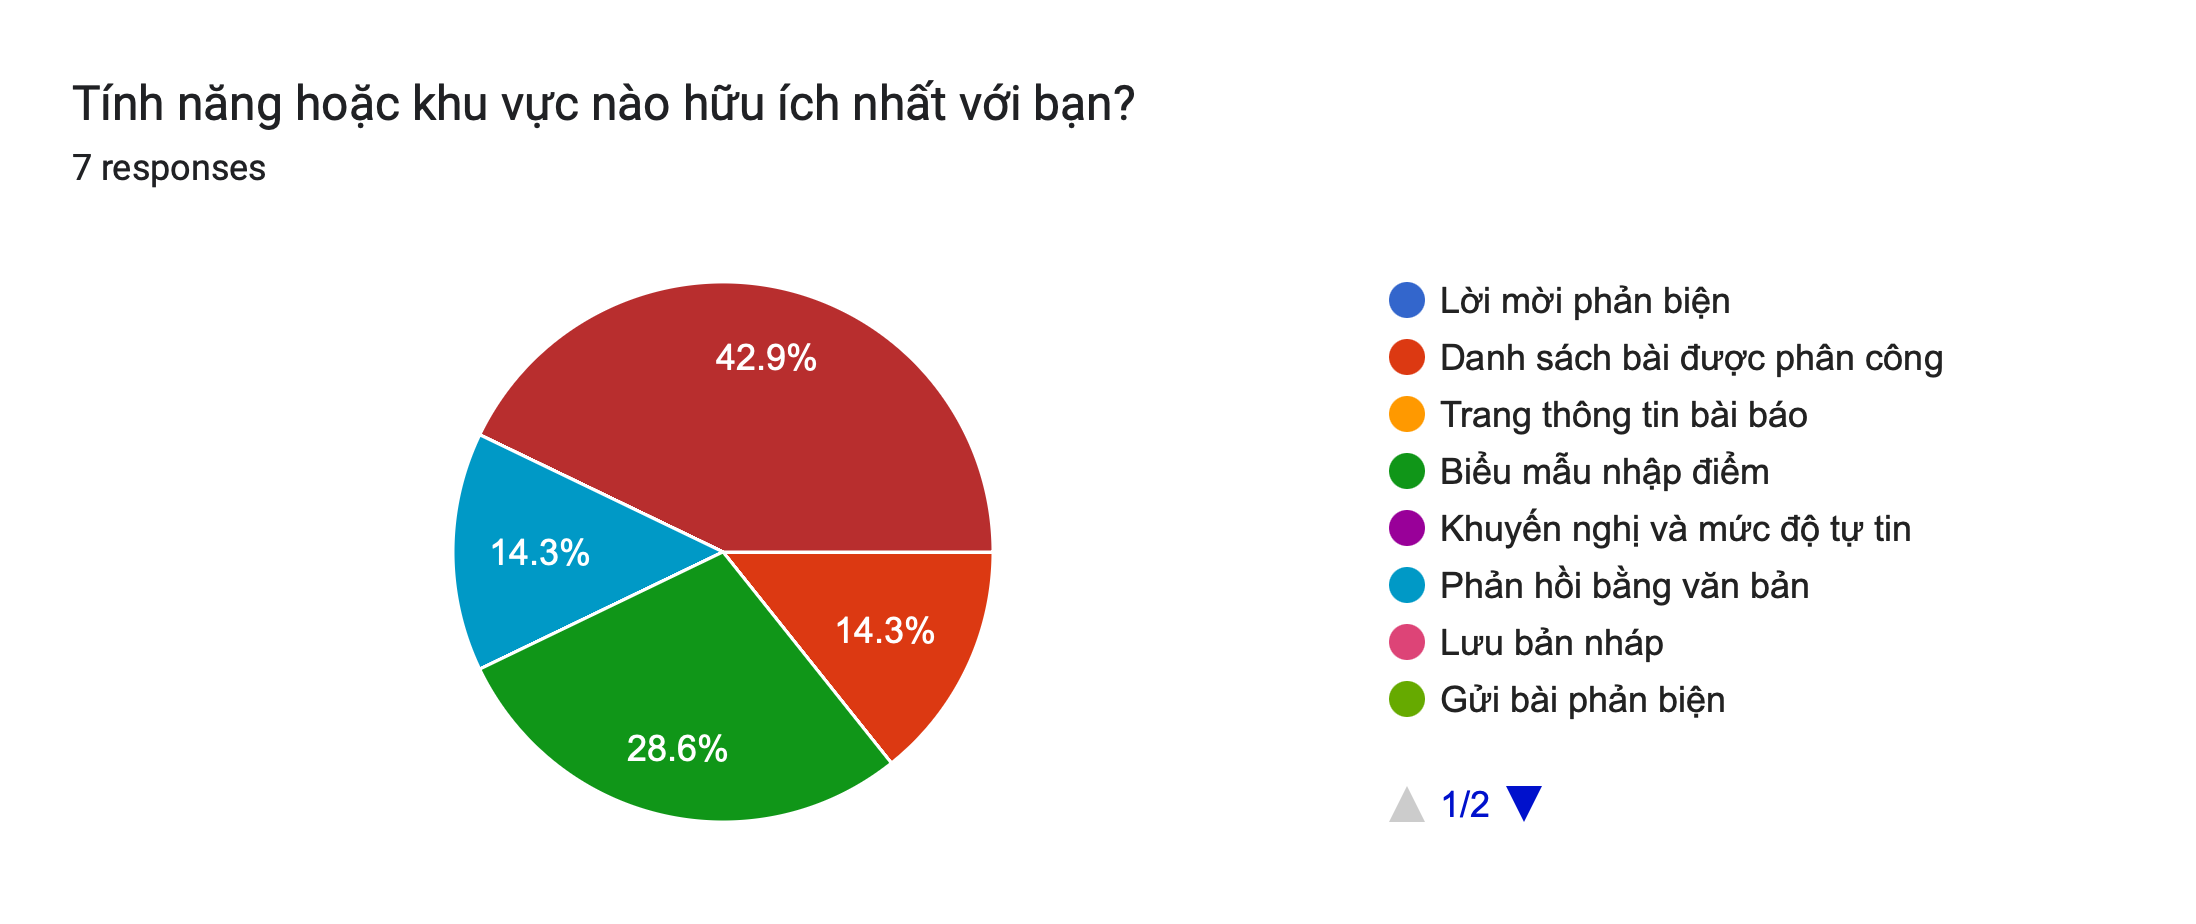
\includegraphics[width=0.9\textwidth]{images/chapter_4_reviewer.png}
    \caption{Kết quả khảo sát sau sử dụng theo vai trò Phản biện viên}
    \label{fig:ch4-uat-reviewer-results}
\end{figure}

\subsection{Kết quả theo vai trò Tác giả}

Với cỡ mẫu lớn nhất, điểm hài lòng tổng thể trung bình của Tác giả đạt 3,89/5,00; 67/76 người (88,2\%) chọn ``hài lòng'' hoặc ``rất hài lòng''. Submission Autofill được 47/76 Tác giả (61,8\%) chọn là tính năng hữu ích nhất. Ngoài ra, 69/76 người đồng ý hoặc hoàn toàn đồng ý với nhận định rằng kết quả AI giúp giảm thao tác thủ công hoặc tiết kiệm thời gian. Đây là đánh giá cảm nhận, không phải phép đo số phút tiết kiệm. Phản hồi mở vẫn yêu cầu cải thiện khả năng trích xuất khi định dạng tác giả phức tạp hoặc tệp PDF chứa nhiều công thức; vì vậy, bản nháp phải tiếp tục cho phép Tác giả kiểm tra và chỉnh sửa.


\begin{figure}[H]
    \centering
    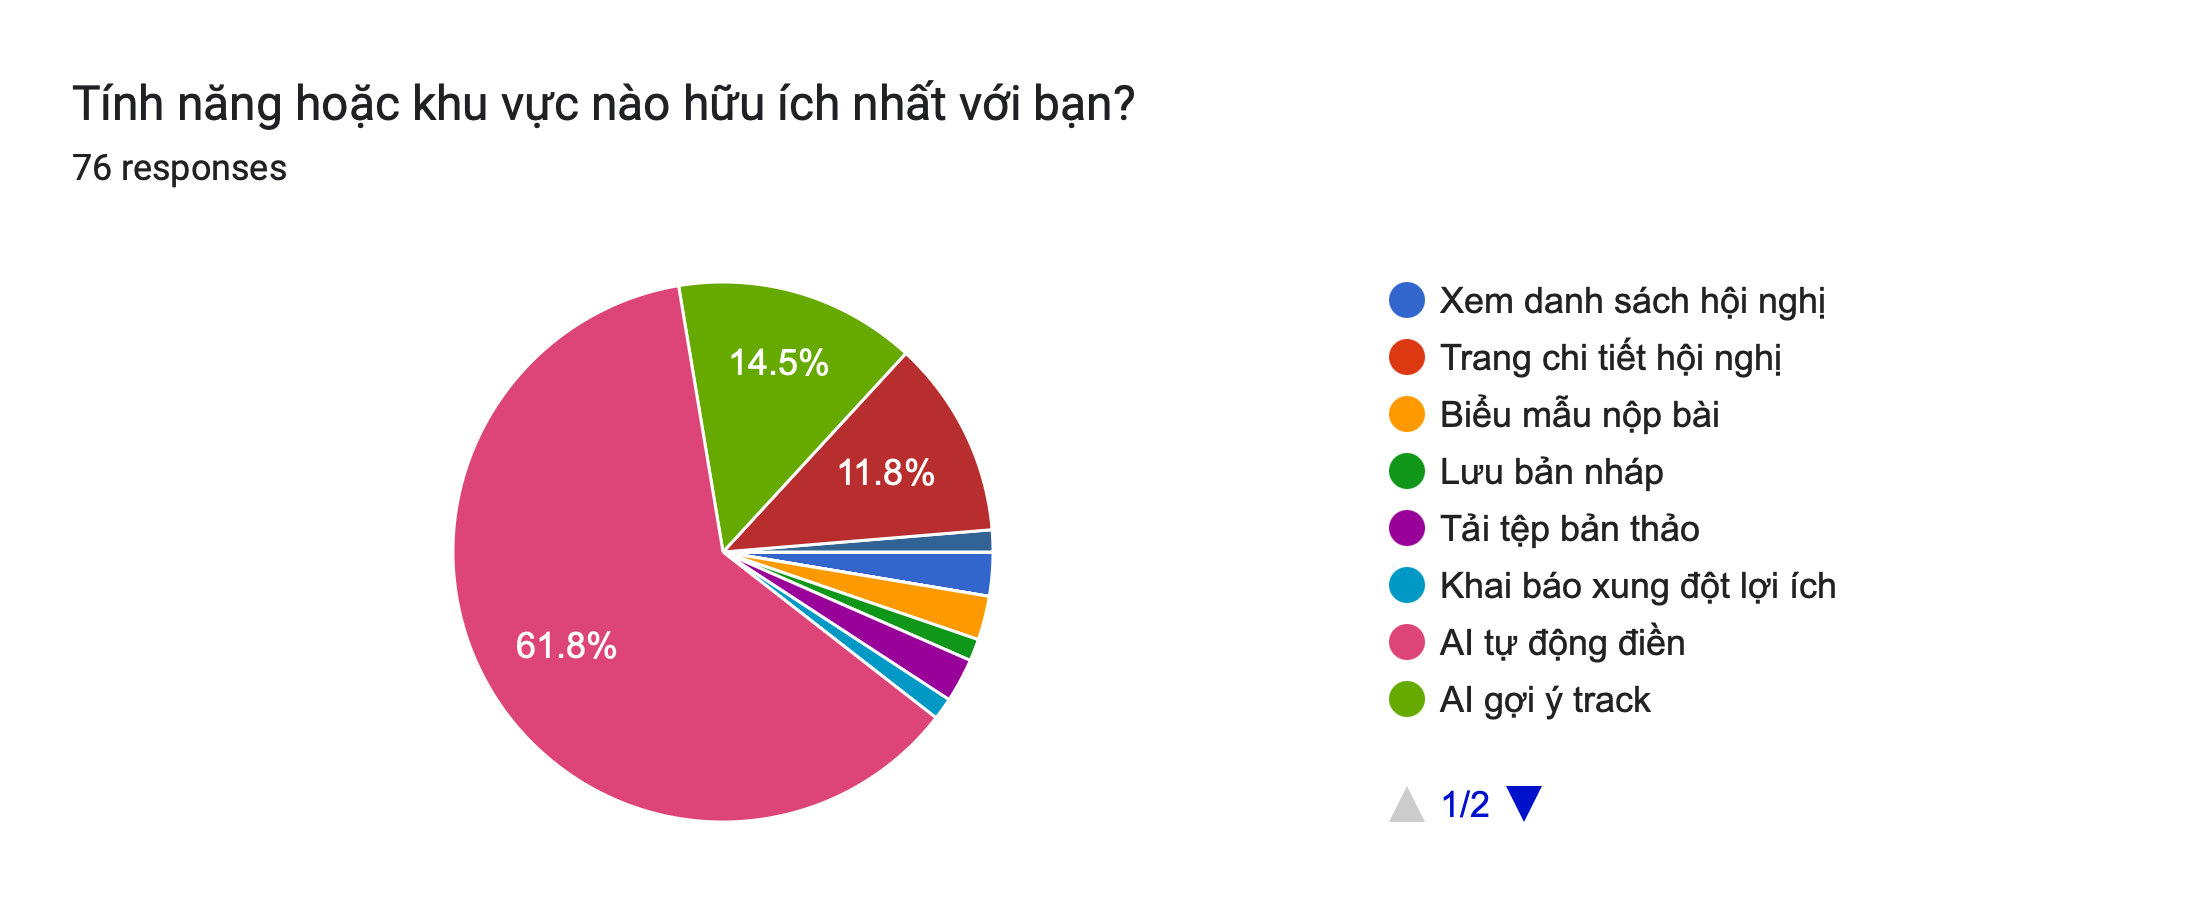
\includegraphics[width=0.9\textwidth]{images/chapter_4_author_1.png}
    \caption{Kết quả khảo sát sau sử dụng theo vai trò Tác giả: tính năng hữu ích}
    \label{fig:ch4-uat-author-satisfaction}
\end{figure}

\begin{figure}[H]
    \centering
    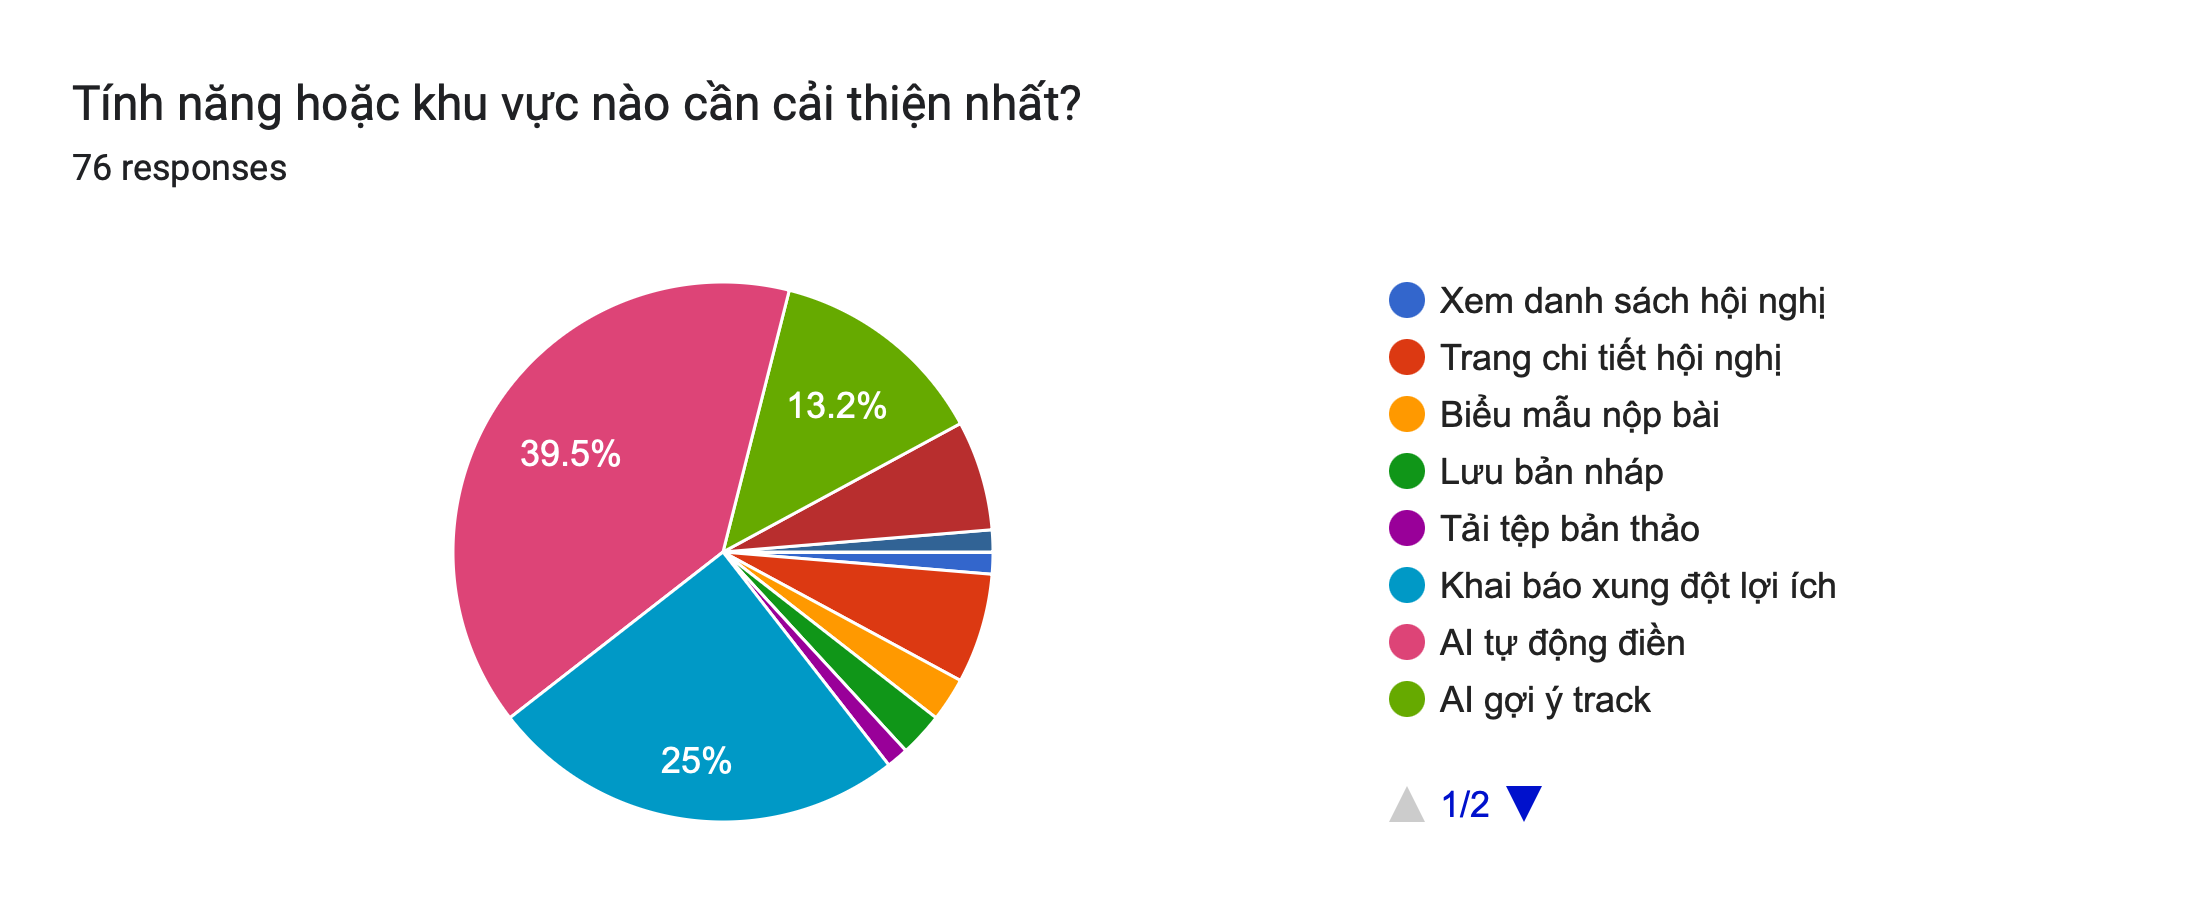
\includegraphics[width=0.9\textwidth]{images/chapter_4_author_2.png}
    \caption{Kết quả khảo sát sau sử dụng theo vai trò Tác giả: tính năng được người dùng quan tâm và đề xuất cải thiện}
    \label{fig:ch4-uat-author-useful-features}
\end{figure}

\begin{figure}[H]
    \centering
    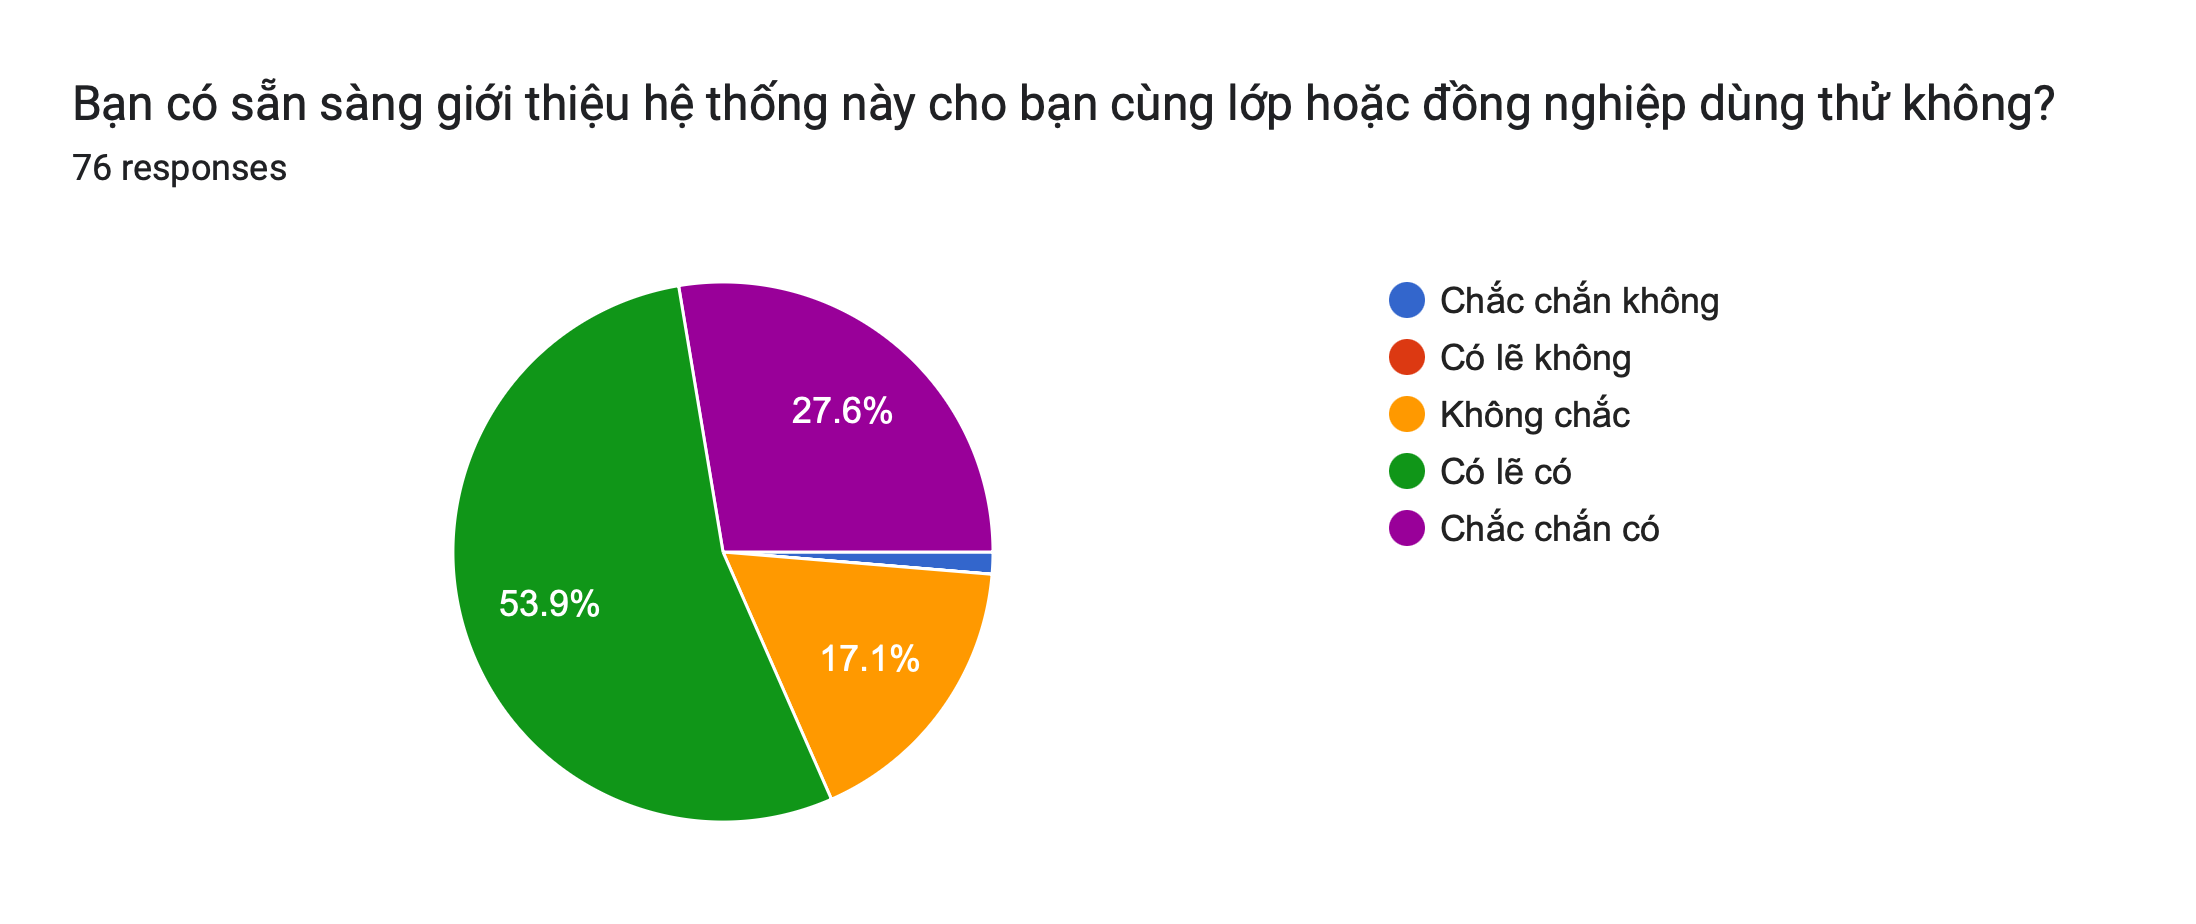
\includegraphics[width=0.9\textwidth]{images/chapter_4_author_3.png}
    \caption{Kết quả khảo sát sau sử dụng theo vai trò Tác giả: sẵn sàng giới thiệu nền tảng cho người quen}
    \label{fig:ch4-uat-author-improvements}
\end{figure}

\subsection{Tổng hợp xuyên vai trò}

\textbf{Đánh giá tổng quan:} 73/91 phản hồi (80,2\%) chọn ``có lẽ có'' hoặc ``chắc chắn có'' khi được hỏi về việc giới thiệu nền tảng cho bạn cùng lớp hoặc đồng nghiệp. Theo vai trò, tỷ lệ này là 62/76 ở nhóm Tác giả, 6/7 ở nhóm Phản biện viên và 5/8 ở nhóm Chủ tọa. Kết quả toàn mẫu chịu ảnh hưởng lớn từ nhóm Tác giả vì nhóm này chiếm 83,5\% mẫu phân tích; tỷ lệ giữa các vai trò không nên được dùng để xếp hạng do cỡ mẫu chênh lệch.

\textbf{Cảm nhận về giảm thao tác:} 69/76 Tác giả, 5/7 Phản biện viên và 7/8 phản hồi Chủ tọa đồng ý hoặc hoàn toàn đồng ý rằng kết quả AI giúp giảm thao tác thủ công hoặc tiết kiệm thời gian. Câu hỏi không đo thời gian thực hiện nhiệm vụ, nên báo cáo không quy đổi kết quả thành số phút hoặc phần trăm thời gian tiết kiệm.

Các chỉ số khảo sát không thay thế thử nghiệm kỹ thuật, nhưng giúp nối kết quả vận hành với cảm nhận của mẫu người dùng sau khi trải nghiệm hệ thống.

\textbf{Đề xuất cải thiện theo mức độ ưu tiên:}

Mặc dù Submission Autofill được đánh giá hữu ích nhất, tính năng này vẫn cần cải thiện khả năng trích xuất đối với bài có định dạng PDF phi chuẩn, nhiều ký hiệu toán học hoặc cấu trúc tác giả phức tạp, chẳng hạn bài báo y khoa. Điểm hài lòng đối với các tính năng dành cho Chủ tọa và Phản biện viên ở mức cao trong mẫu khảo sát, nhưng cỡ mẫu của hai nhóm còn nhỏ. Riêng ở nhóm Chủ tọa, tỷ lệ người trả lời nêu điểm gây khó chịu cho thấy lần đánh giá tiếp theo cần ưu tiên độ tin cậy của gợi ý AI, tính minh bạch trong cách sử dụng dữ liệu và khả năng bỏ qua hoặc sửa gợi ý; đồng thời, nhóm cần mở rộng mẫu bằng quy trình tuyển chọn có thể kiểm chứng mà vẫn bảo vệ danh tính người tham gia.

\section{Tổng hợp kết quả đánh giá}

Chương này trả lời câu hỏi trách nhiệm theo từng lớp thay vì đưa ra một phán quyết chung về AI. Do không có ngưỡng thành công được xác lập trước cho mọi chỉ số, bảng tổng hợp phân biệt bằng chứng trực tiếp, chỉ số gián tiếp và phần chưa đo; các nhãn này mô tả quan hệ giữa phép đo và nhận định, không xếp hạng chất lượng sản phẩm.

\begin{PrismLongTable}
\begin{longtable}{|P{0.18\textwidth}|P{0.25\textwidth}|P{0.19\textwidth}|P{0.30\textwidth}|}
  \caption{Mức kết luận theo trách nhiệm và bằng chứng}\LongTableCaptionSpace
  \hline
  \TableHeader{Nhận định/trách nhiệm} & \TableHeader{Bằng chứng chính} & \TableHeader{Mức kết luận} & \TableHeader{Giới hạn quyết định} \\ \hline
  \endfirsthead
  \LongTableHeaderBorder
  \TableHeader{Nhận định/trách nhiệm} & \TableHeader{Bằng chứng chính} & \TableHeader{Mức kết luận} & \TableHeader{Giới hạn quyết định} \\ \hline
  \endhead
  \LongTableFooterBorder
  \endfoot
  Hiệu năng các endpoint đã chọn & Ba kịch bản k6; p95 dưới 120 ms; 0\% lỗi yêu cầu & Có bằng chứng trực tiếp trong cấu hình thử nghiệm & Chỉ đo ba endpoint đọc, gợi ý và kiểm tra; không thay thế kiểm thử chức năng toàn vòng đời hoặc chứng minh hệ thống sẵn sàng triển khai thực tế \\ \hline
  Truy hồi hồ sơ tác giả và hành vi phân công & Trên dữ liệu tổng hợp: phép leave-one-out theo tác giả, các phương pháp cơ sở, MRR 0,392; Hit@5 = 55\%; Hit@10 = 65\%; các chỉ số nội tại của phân công & Chỉ có chỉ số gián tiếp & Nhãn tác giả gốc đo quan hệ chủ đề, không đo mức độ phù hợp của phản biện viên; chưa có dữ liệu về mức chấp nhận của Chủ tọa \\ \hline
  Phát hiện xung đột lợi ích & Microbenchmark cho ca tự gán và xung đột đã khai báo; không có ca tự gán trong tập phân công & Chưa đo chất lượng xung đột lợi ích đa tầng & Chưa kiểm thử lớp đồ thị hoặc xây dựng tập cặp xung đột do chuyên gia gán nhãn \\ \hline
  Submission Autofill và Submission Gating theo luật & Siêu dữ liệu của 1.127 bài; 8/8 ca kiểm tra luật; 24 ca cảnh báo mềm & Có bằng chứng trực tiếp cho siêu dữ liệu và bộ ca kiểm tra luật & Các trường phức tạp có trường hợp thất bại; gợi ý chuyên đề và cảnh báo mềm thiếu nhãn chuyên gia; chưa đo số thao tác \\ \hline
  Initial Analysis & Điểm TCA thăm dò trên 1.097 gói; 96,22\% trích dẫn bám nguồn và 69,86\% điểm cần lưu ý trung thực theo bộ chấm & Chỉ có chỉ số gián tiếp & TCA/NLI chưa hiệu chuẩn; đầu ra có thể ảnh hưởng nội dung phản biện; chưa đo mức độ hữu ích, mức độ phụ thuộc hoặc sự phù hợp với chính sách \\ \hline
  Quality Auditor & 3.658 lượt kiểm tra; 2.637--3.472 đơn vị chấm tùy chỉ số; 46,99\% vừa bám nguồn vừa hợp lệ & Chưa đáp ứng ranh giới trách nhiệm & Nhiễu cao; phát hiện xác suất có thể chặn gửi và chưa có quyền ghi đè; chưa đo tỷ lệ chặn sai \\ \hline
  Chair Copilot & Điểm TCA thăm dò; cơ sở bằng chứng 87,34\%; bất đồng 87,11\%; UAT Chủ tọa có tám phản hồi ẩn danh & Chỉ có chỉ số gián tiếp và cảm nhận theo câu hỏi gộp & UAT không tách riêng luồng này, không đo độ đúng quyết định hoặc thiên lệch tự động hóa; cỡ mẫu nhỏ và hồ sơ người tham gia không được kiểm chứng độc lập \\ \hline
  Chatbot theo quyền và phạm vi & 40 hội thoại; không lộ dữ liệu trong kịch bản quyền; một lượt viết báo cáo ngoài phạm vi & Có bằng chứng theo kịch bản, kết quả không đồng đều & 31/128 lượt gọi công cụ thất bại; kiểm soát nội dung ngoài phạm vi đã thất bại một biến thể; không phải kiểm toán bảo mật \\ \hline
  Giảm phụ thuộc vào AI & Đường thao tác thủ công và ranh giới kiến trúc được mô tả & Chưa đo đầu cuối & Chưa có thử nghiệm chèn lỗi khi yêu cầu đến dịch vụ AI bị timeout hoặc ngừng hoạt động \\ \hline
  Trải nghiệm theo vai trò & UAT 91 phản hồi có đồng thuận và đủ dữ liệu cho các chỉ số chính, gồm 76 phản hồi Tác giả, 7 phản hồi Phản biện viên và 8 phản hồi Chủ tọa & Chỉ có bằng chứng cảm nhận, chủ yếu từ Tác giả & Mẫu thuận tiện, cỡ mẫu nhỏ ở hai vai trò chuyên môn; phản hồi Chủ tọa ẩn danh không cho phép kiểm chứng độc lập đặc điểm mẫu; chưa đo thời gian, hành vi hoàn thành nhiệm vụ hoặc thiên lệch tự động hóa \\ \hline
  Quản trị dữ liệu nhà cung cấp ngoài & Phân quyền cấp ứng dụng & Chưa đo & Chưa kiểm toán lưu giữ, huấn luyện và vùng cư trú; không đủ cơ sở dùng dữ liệu mật trong hội nghị thật \\ \hline
\end{longtable}
\end{PrismLongTable}

\subsection{Mức độ đáp ứng nhu cầu ban đầu}

Đối chiếu với Chương 1 và Chương 2, lớp nghiệp vụ có bằng chứng hiệu năng cho các endpoint đã thử, nhưng chưa có bằng chứng chức năng đầu cuối cho toàn bộ vòng đời. Trên dữ liệu tổng hợp, phương pháp xếp hạng Jaccard truy hồi hồ sơ tác giả gốc tốt hơn phương pháp cơ sở ngẫu nhiên; phép thử chưa đo mức độ phù hợp của phản biện viên. Thủ tục phân công đạt độ phủ đủ hai người ở 65,9\% số bài; 23,3\% số bài phải dùng lượt dự phòng không còn ngưỡng điểm và giới hạn tải tối đa. Với xung đột lợi ích, microbenchmark chỉ bao phủ ca tự gán và xung đột đã khai báo; chất lượng của lớp đồ thị và khả năng phát hiện quan hệ ẩn chưa được đo.

Lớp AI cho kết quả khác nhau theo từng tác vụ. Submission Autofill có bằng chứng trực tiếp nhất ở khả năng trích xuất siêu dữ liệu. Submission Gating đạt 8/8 ca kiểm tra luật, nhưng cảnh báo mềm chưa có nhãn chuyên gia. Reviewer Initial Analysis tạo được các nhận định có căn cứ trong nguồn, song các điểm cần chú ý vẫn có rủi ro. Review Quality Auditor có mức nhiễu cao. Chair Decision Copilot tạo bản tổng hợp có mức độ bám nguồn đo được, nhưng chưa có đánh giá chuyên gia về tác động đến quyết định. Chatbot Agent không làm lộ dữ liệu trong kịch bản phân quyền đã chạy, nhưng kiểm soát nội dung ngoài phạm vi thất bại ở một biến thể và tỷ lệ lỗi khi gọi công cụ còn đáng kể.

UAT ghi nhận cảm nhận tích cực về trải nghiệm, đặc biệt ở nhóm Tác giả, nhưng không chứng minh quan hệ nhân quả đối với thời gian tiết kiệm hoặc chất lượng quyết định. Nhìn chung, ConferenceSpace đã triển khai mô hình phân chia trách nhiệm theo ba lớp và tạo chuỗi bằng chứng ban đầu cho từng trách nhiệm. Bằng chứng hiện có chưa hỗ trợ các nhận định về khả năng cô lập lỗi AI đầu cuối, quản trị toàn vòng đời dữ liệu của nhà cung cấp, thiên lệch tự động hóa, ưu thế so với nền tảng khác hoặc mức độ sẵn sàng để triển khai thực tế.

\subsection{Các phát hiện nhất quán giữa thử nghiệm và khảo sát người dùng}

Phân tích đối chiếu giữa dữ liệu kỹ thuật và phản hồi người dùng cho thấy một số phát hiện nhất quán quan trọng.

\textbf{Submission Autofill là luồng có bằng chứng định lượng trực tiếp nhất.} Thử nghiệm siêu dữ liệu cho thấy hệ thống đạt tỷ lệ đối sánh cao ở các trường ngắn và có cấu trúc rõ; phản hồi của người dùng tại Mục 4.7 cũng đánh giá tích cực khả năng giảm thao tác nhập liệu. Cả hai nguồn bằng chứng đều chỉ ra một giới hạn: người dùng vẫn phải kiểm tra kỹ các tài liệu có định dạng phức tạp, nhiều tác giả hoặc nhiều ký hiệu toán học.

\textbf{Reviewer Initial Analysis có chỉ số bám nguồn nhưng chưa được xác nhận về ranh giới trách nhiệm.} Bộ chấm ghi nhận tỷ lệ trích dẫn bám nguồn cao, nhưng điểm cần lưu ý, điểm mạnh, điểm yếu và gợi ý vẫn có thể định hướng nhận định. Câu hỏi UAT gộp nhiều thành phần và chỉ có bảy Phản biện viên, nên không thể dùng để xác nhận riêng mức độ hữu ích, sự phù hợp với chính sách hoặc ảnh hưởng đến chất lượng phản biện.

\textbf{Chair Decision Copilot có bằng chứng về mức bám nguồn của bản tổng hợp.} TCA ghi nhận cơ sở bằng chứng và bản tổng hợp các điểm bất đồng đạt khoảng 87\%. Trong UAT dành cho Chủ tọa, 7/8 phản hồi đồng ý rằng công cụ AI chỉ hỗ trợ con người, cung cấp đủ căn cứ cho gợi ý và cho phép người dùng thoải mái đặt nghi vấn hoặc bỏ qua kết quả. Tuy nhiên, câu hỏi gộp nhiều công cụ AI và tám phản hồi được thu thập ẩn danh, nên kết quả chỉ phản ánh cảm nhận chung của vai trò này, không xác nhận riêng Chair Decision Copilot. Kết quả chưa chứng minh luồng giúp đọc nhanh hơn, cải thiện chất lượng quyết định hoặc không tạo thiên lệch tự động hóa; Chủ tọa vẫn phải kiểm tra nguồn và chịu trách nhiệm quyết định.

\textbf{Số liệu kỹ thuật và phản hồi người dùng cùng cho thấy các điểm nghẽn vận hành.} Thử nghiệm ghi nhận một số trường hợp có độ trễ cao ở các luồng, nhiều lần gọi công cụ thất bại ở Chatbot Agent và tỷ lệ phát hiện nhiễu cao ở Review Quality Auditor. Giao diện cần thể hiện các vấn đề này bằng cách hiển thị trạng thái xử lý, đánh dấu mức tin cậy, gom nhóm phát hiện và cho phép người dùng kiểm tra nguồn.

\subsection{Hạn chế của kết quả thực nghiệm}

Các hạn chế ghi nhận trong thực nghiệm giới hạn phạm vi kết luận của chương.

\textbf{Thiếu nhãn chuyên gia cho một số luồng.} Gợi ý chuyên đề trong Submission Autofill mới ghi nhận tỷ lệ hoàn tất và tỷ lệ chuyên đề không hợp lệ 0,00\%, chưa cung cấp bằng chứng về độ chính xác trong $k$ vị trí đầu. Phần cảnh báo mềm của Submission Gating cũng chưa được con người rà soát từng cảnh báo để xác định mức độ bám bằng chứng, khả năng hỗ trợ chỉnh sửa và mức độ nghiêm trọng. Chair Decision Copilot chưa được đối chiếu với quyết định chấp nhận hoặc từ chối của Chủ tọa, nên dữ liệu hiện có không cho phép kết luận về độ chính xác của quyết định cuối cùng.

\textbf{Một số luồng vi phạm hoặc chưa được xác nhận về ranh giới trách nhiệm.} Review Quality Auditor có độ trung thực 58,28\% và tỷ lệ vừa bám nguồn vừa hợp lệ 46,99\%, nhưng vẫn có thể chặn gửi mà không có quyền ghi đè; cơ chế hiện tại chưa đáp ứng nguyên tắc tư vấn. Reviewer Initial Analysis có độ trung thực của điểm cần lưu ý 69,86\% và tạo nội dung gần với một phần bản phản biện; báo cáo chưa có cơ sở khẳng định chức năng này chỉ điều hướng trung lập hoặc phù hợp với mọi chính sách hội nghị.

\textbf{Phương pháp TCA cung cấp bộ chỉ số tự động gián tiếp và không thay thế chuyên gia.} Suy luận ngôn ngữ tự nhiên (NLI) có thể bỏ sót mệnh đề đúng nhưng diễn đạt khác, hoặc đánh giá thấp các suy luận kỹ thuật phức tạp. Vì vậy, các chỉ số độ trung thực, độ phủ và Additionality nên được đọc như tín hiệu đánh giá trên quy mô lớn sau khi đã có kết quả, không phải phán quyết cuối cùng về chất lượng học thuật.

\textbf{Cơ chế xử lý độ trễ và vận hành cần được hoàn thiện trước khi triển khai.} Một số luồng có trường hợp vượt 100 giây. Chatbot Agent có 31/128 lượt gọi công cụ thất bại và thời gian trung bình đến câu trả lời hoàn chỉnh đầu tiên là 23,02 giây. Hệ thống cần hàng đợi, cơ chế thử lại, thông tin về tiến độ xử lý và thông báo rõ hơn về lỗi hoặc quyền truy cập. Chương chưa có thử nghiệm chạy bền, thử nghiệm phân tán hoặc thử nghiệm chèn lỗi đầu cuối.

\textbf{Đối sánh phản biện viên vẫn cần dữ liệu thực tế từ Chủ tọa.} Trên bộ dữ liệu tổng hợp, phép leave-one-out cho thấy thuật toán truy hồi hồ sơ tác giả gốc tốt hơn đường cơ sở ngẫu nhiên. Kết quả này không thay thế đánh giá bằng dữ liệu phân công thật của Chủ tọa hoặc tỷ lệ chấp nhận đề xuất trong vận hành thực tế.

\textbf{Phạm vi ngôn ngữ và bối cảnh còn hẹp.} Thử nghiệm chủ yếu dựa trên bài báo tiếng Anh và dữ liệu hội nghị từ OpenReview. Hiệu quả với bài tiếng Việt, hội nghị nhỏ không dùng OpenReview hoặc quy trình phản biện có chính sách khác vẫn cần được đánh giá thêm.

\textbf{Các ranh giới quản trị chưa được kiểm toán.} Cơ chế phân quyền ở cấp ứng dụng không cho biết nhà cung cấp AI lưu giữ dữ liệu trong bao lâu, có dùng dữ liệu để huấn luyện hay không hoặc đặt dữ liệu tại khu vực nào. Thử nghiệm cũng chưa đo thiên lệch tự động hóa, chưa so sánh trực tiếp với PeerSubmit và chưa đánh giá hệ thống trong một hội nghị vận hành thực tế.

\textbf{UAT chưa hỗ trợ suy rộng thống kê cho các vai trò chuyên môn.} Nguồn lực của nhóm và yêu cầu kinh nghiệm đối với Phản biện viên, đặc biệt là Chủ tọa, làm hạn chế khả năng tuyển mẫu lớn. Hình thức ẩn danh giúp giảm rào cản tham gia nhưng khiến nhóm không thể kiểm chứng độc lập danh tính, tính duy nhất và hồ sơ chuyên môn từ tệp xuất. Vì vậy, các tỷ lệ UAT theo hai vai trò này chỉ mô tả mẫu tham gia và không được dùng để kết luận cho quần thể rộng hơn.

Tóm lại, Chương 4 xác nhận hiệu năng của các endpoint đã chọn, mức độ khớp của siêu dữ liệu do Submission Autofill tạo và hành vi của bộ ca kiểm tra luật trong cấu hình thử nghiệm. Các phép truy hồi chủ đề và TCA chỉ cung cấp chỉ số gián tiếp, còn UAT chỉ phản ánh cảm nhận của mẫu tham gia. Chất lượng phát hiện xung đột lợi ích đa tầng, tính đúng đắn của toàn bộ vòng đời, hiệu lực kiểm soát của con người và cơ chế quản trị dữ liệu chưa được đo đầy đủ. Review Quality Auditor chưa tuân thủ ranh giới tư vấn vì phát hiện theo xác suất vẫn có thể chặn thao tác gửi. Do đó, báo cáo chỉ kết luận rằng nhóm đã triển khai mô hình trách nhiệm và thu được bằng chứng theo từng tác vụ; dữ liệu hiện có không xác nhận toàn bộ cách phân bổ trách nhiệm đã thành công hoặc hệ thống đã sẵn sàng để triển khai thực tế.